% Centro de Estadística y Matemática Aplicada
% Universidad Simón Bolívar
% Plantilla LaTeX para manuscritos (tesis y pasantías)
% pregrado y postgrado
%
% Andrés M. Sajo-Castelli
% Carlos Contreras
%
% 15 Abril 2015 -- primera versión pública
% ...
% 11 Mayo 2018 --- Se agrega bibliografía en castellano via babelbib
%
\documentclass[pregrado]{tesis-usb}

% paquetes
\usepackage[utf8]{inputenc}
\usepackage{verbatim}
\usepackage{acronym}
\usepackage{amsmath}
\usepackage{amsfonts}
\usepackage{amssymb}
\usepackage{array}
% \usepackage{hyperref}
%acontinuación lo que se necesita para hacer tablas bonitas
\usepackage{booktabs} 
\usepackage{multirow}
\usepackage{siunitx}

% estilo de las referencias
\usepackage[fixlanguage]{babelbib-and}\selectbiblanguage{spanish}
\usepackage{url}
\bibliographystyle{babplain-lf}

%para agregar varias imagenes en una sola figura
\usepackage{graphicx}
\usepackage{subcaption}

%para ponerle color al texto
\usepackage{xcolor}

\usepackage{geometry}
\usepackage{hyperref}
\hypersetup{colorlinks=true, urlcolor=blue, linkcolor=black}
\usepackage{caption}

\usepackage{rotating} 


\autor{María Laura Rojas González}
\autori{M. Rojas}
\usbid{19-10256}
\titulo{Efectos de la densidad de energía gravitacional sobre la velocidad de la luz: verificación experimental de la Hipótesis de Céspedes-Curé}
\fecha{Junio~de~2026}
\agno{2026}
\fechadefensa{30~de~Junio~de~2026}
\tutor{Dr. Eduardo Greaves}
% \usarcotutor
\cotutor{Nombre y Apellido \mbox{(Afiliaci\'on)}} 
\trabajo{Trabajo de grado}
\coord{Física}
\grado{Licenciado en física}
\carrera{Física}
\programa{Nombre del Programa}
\juradouno{Nombre y Apellido}
\juradodos{Nombre y Apellido \mbox{(Afiliaci\'on)}}
\juradotres{Nombre y Apellido}

% Cambia comillas simple por comilla cerrada en ambiente verbatim 
\makeatletter
\let \@sverbatim \@verbatim
\def \@verbatim {\@sverbatim \verbatimplus}
{\catcode`'=13 \gdef \verbatimplus{\catcode`'=13 \chardef '=13 }} 
\makeatother
%esto permite que las subsubsection aparezcan en el indice
\setcounter{tocdepth}{3} 
%sto permite que las subsubsection se enumeren
\setcounter{secnumdepth}{3}

\begin{document}

\frontmatter
\maketitle
\chapter*{Dedicatoria}

 A mi, por no rendirme a persar de la adversidad.

\chapter*{Agradecimientos}

 %Eduardo Greaves, Fernando anzola, Laboratorio de Fisica Nuclear, Instituto IDT+i, Desiree Aguero, Carmelo García, Marycarmen Rivas, por prestarme todo su apoyo tanto técnico y material como emocional Orfeón Universitario, familia. A la UDO por comenzar mi formación y a la simon por recibirme con los brazos abiertos.

 Al profesor Eduardo Greaves por su guía en estos años y por brindarme oportunidad de hacer ciencia dentro de este tema tan fascinante; su labor, ingenio y actitud  me inspiran a ser mejor profesional.

 Al Laboratorio de Física Nuclear, Instituto IDT+i, al profesor Fernando Anzola y a la ingeniera Desiree Aguero, por prestarme toda su colaboración técnica y material, sin ella no habría podido realizarse este trabajo.

 Al Orfeón Universitario Simón Bolivar por recibirme desde el primer día y enseñarme los valores de la comunidad universitaria usebista.

 A los amigos que la física puso en mi camino, por la ayuda brindada en la carrera pero sobretodo por los momentos vividos que siempre atesoraré.

 A mi mejor amiga, Marycarmen Rivas, gracias por estar ahí para mí en los momentos de mayor estrés y por escucharme siempre.

 A mi compañero de vida, Carmelo García, gracias por quererme, motivarme, apoyarme y creer en mí incluso más que yo misma. 

 A mi familia, mis padres, mis hermanos y mi sobrino, cuyo cariño me ha servido de motor durante toda mi vida. Especial agradecimiento a mi mamá, Damelis, quien me apoyó desde el primer momento en la carrera, no solo una sino dos veces.

 Finalmente, a la UDO por permitirme comenzar mi formación academica, y a la USB por recibirme con los brazos abiertos.






\begin{resumen}
     Es una exposici\'on clara del tema tratado en el trabajo.
%      Para redactar el **Resumen** de tu libro de tesis siguiendo estrictamente los lineamientos del Decanato de Estudios Profesionales (DEP) de la USB, debes tener en cuenta que este se escribe en **un único párrafo continuo de máximo 250 palabras**,, debe ir en la página romana **"v"**,, y **no debe contener citas bibliográficas** de ningún tipo,. Además, cualquier acrónimo que utilices por primera vez debe definirse inmediatamente entre paréntesis (por ejemplo, *Hipótesis de Céspedes-Curé (HCC)*),.

% A continuación, te presento el esquema secuencial de las ideas que debes incluir y el orden exacto en el que deben fluir dentro de ese único párrafo para garantizar coherencia, rigor científico y apego a la normativa:

% ---

% # ESQUEMA SECUENCIAL PARA EL PÁRRAFO ÚNICO DE RESUMEN

% ### 1. Contexto y Enunciado del Paradigma (Sentencias 1 y 2)
% *   **Idea a incluir:** Comienza presentando de forma concisa el marco teórico y la hipótesis física que busca verificar tu investigación.
% *   **Detalles a redactar:** Enuncia la Hipótesis de Céspedes-Curé (HCC), la cual postula que la velocidad de la luz (\\(c\\)) no es una constante universal en el vacío, sino que varía localmente en función de la densidad de energía gravitacional del medio (\\(c = k\sqrt{\rho}\\)).

% ### 2. Objetivo Principal del Trabajo (Sentencia 3)
% *   **Idea a incluir:** Define claramente qué hiciste en tu proyecto para abordar esta hipótesis.
% *   **Detalles a redactar:** Declara el objetivo de diseñar, construir y evaluar un sistema experimental modular indirecto de alta precisión, basado en circuitos resonantes RLC, para medir variaciones infinitesimales de la permitividad eléctrica del vacío (\\(\epsilon_0\\)) como transductor de las fluctuaciones gravitacionales en la superficie terrestre.

% ### 3. Metodología e Implementación de Ingeniería (Sentencias 4 y 5)
% *   **Idea a incluir:** Resume el diseño de hardware, los módulos electrónicos implementados y el control de variables ambientales.
% *   **Detalles a redactar:** Describe la arquitectura del montaje: el uso de un oscilador AD9833 controlado por un microcontrolador Arduino para barridos de frecuencia estables, un módulo de lectura con rectificador analógico y conversión digital (mediante el ADS1115), y un sistema de control térmico activo autónomo diseñado para neutralizar perturbaciones de temperatura ambiental en el circuito resonante.

% ### 4. Tratamiento Matemático de los Datos (Sentencia 6)
% *   **Idea a incluir:** Explica brevemente cómo se procesaron matemáticamente los datos para obtener la máxima precisión posible.
% *   **Detalles a redactar:** Menciona el desarrollo del software en Python para la adquisición de datos y la implementación del algoritmo de Regresión Ortogonal de Distancias (ODR) como método estadístico para determinar la frecuencia de resonancia (\\(f_0\\)) minimizando la incertidumbre instrumental de ambos ejes.

% ### 5. Resultados Clave Obtenidos (Sentencias 7 y 8)
% *   **Idea a incluir:** Sintetiza los hallazgos experimentales más importantes y contrasta los prototipos desarrollados de manera cuantitativa.
% *   **Detalles a redactar:** Expón que la configuración en paralelo superó con creces a la de serie en términos de estabilidad de la curva, alcanzando un error relativo mínimo de apenas **0,0036%** frente al **0,34%** de la serie. Sincera que, aunque los prototipos actuales demostraron gran robustez instrumental y térmica, se requiere de mayor resolución para discernir con certeza los corrimientos de frecuencia esperados en las tres altitudes geográficas propuestas (Carmen de Urea, USB y el Teleférico).

% ### 6. Conclusión y Futuro Tecnológico (Sentencia 9)
% *   **Idea a incluir:** Cierra con el impacto del trabajo y la ruta de experimentación avanzada propuesta.
% *   **Detalles a redactar:** Concluye validando el método indirecto RLC como una alternativa viable frente al método directo con láser (Experimento I) y propone la transición tecnológica futura hacia la plataforma Red Pitaya y el acoplamiento por inducción para alcanzar la novena cifra significativa de resolución requerida.

% ---

% ### Palabras clave (Al final de la página, separadas por comas)
% Debes incluir al final, fuera del párrafo del resumen, las siguientes 5 palabras clave de tu investigación,,:
% > **Palabras clave:** hipótesis de Céspedes-Curé, circuitos resonantes RLC, regresión ortogonal de distancias, estabilidad térmica activa, velocidad de la luz.

\end{resumen}
\tableofcontents
\listoffigures
\listoftables
\useacronyms
\chapter*{Notaci\'on matem\'atica}
\begin{tabular}{ll}
$C$ & Capacitancia\\
%$c$ & Velocidad de la luz\\
$c$, $c_E$ & Velocidad de la luz en la superficie de la tierra, valor aceptado actual $299792458$ m/s\\
$c_i$ & Velocidad de la luz en un punto $i$ de la tierra\\
$G$ & Constante de gravitación universal\\
$g_i$ & Aceleración de la gravedad local en un punto $i$ de la tierra\\
$K_e$ & Constante de Coulomb\\
$L$ & Inductancia\\
$M$ & Masa\\
$M_E$ & Masa de la Tierra\\
$M_S$ & Masa del Sol\\
$n$ & Indice de refración (capítulo 1).\\
$R$ & Resistencia\\
$r$ & Distancia radial\\
$t$ & Tiempo\\
$\epsilon_0$ & Permitividad eléctrica\\
$\mu_0$ & Permeabilidad magnética\\
$\rho$ & Densidad de energía\\
$\rho*$ & Densidad de energía gravitacional debida a las estrellas lejanas\\
$\rho_E$ & Densidad de energía gravitacional en la superficie de la tierra\\
$\rho_s$ & Densidad de energía gravitacional debida al sol




\end{tabular}

\mainmatter
\chapter*{Introducci\'on}
% Aquí hablaremos de la convención actual de la velocidad de la luz como constante, de algunas implicaciones de esto como el uso del efecto doppler para medir distancias, se dejará entre abierta la idea de que el paradigma puede cambiar ...
% Se especificará los temas a tratar en cada capítulo


% ### Parte 1: Contextualización y Paradigma Actual
% *   **Párrafo 1 (El postulado de la velocidad de la luz constante):**
%     *   *De qué hablar:* Introduce el postulado fundamental de la Teoría de la Relatividad Especial de Albert Einstein: la constancia de la velocidad de la luz (\\(c\\)) en el vacío para cualquier observador inercial.
%     *   *Qué mencionar:* Las enormes implicaciones que este supuesto tiene en la física contemporánea y en la metrología (por ejemplo, la definición actual del metro o el uso clásico del efecto Doppler para calcular distancias astronómicas).

En 1905, Albert Einstein publicó la Teoría de la Relatividad Especial, la cual revolucionó la física con dos postulados simples: las leyes de la física son iguales para todos los observadores incerciales, y la luz viaja a una velocidad constante en el vacío. Las implicaciones de estos fueron enormes y llegaron a muchas ramas de la ciencia; por ejemplo, permitió calcular las velocidades de objetos astronómicos mediante el efecto Doppler. Este efecto ya era conocido en ese entonces por su versión sonora, donde si la fuente se acerca o se aleja se puede percibir un cambio en la frecuencia del sonido, haciéndolo más agudo o más grave. Este fenómeno fue fácilmente extrapolado a la luz, donde ahora el cambio de la frecuencia se ve como un cambio en el color: un corrimiento hacia el rojo o al azul. Al conocer la velocidad de la luz, la frecuencia de la señal emitida y la diferencia de dicha frecuencia con respecto a la detectada, es posible conocer la velocidad de desplazamiento de la fuente en dirección radial. Otra implicación de la velocidad de la luz constante está en la actual definición del metro, pues se estableció como la distancia que recorre la luz en un cierto tiempo, convirtiéndolo así en una unidad de distancia que se puede usar universalmente.

% *   **Párrafo 2 (La noción del cambio de paradigma):**
%     *   *De qué hablar:* Plantea de manera elegante e intelectual que, históricamente, los dogmas de la física han cambiado ante nueva evidencia experimental.
%     *   *Qué mencionar:* Introduce la idea de que el vacío podría no ser un escenario pasivo, sino un "medio energético cósmico" con densidades de energía (gravitacionales y electromagnéticas) variables de un punto a otro del universo, lo cual sugiere la posibilidad de que la velocidad de la luz fluctúe según las propiedades de su entorno local.

La física ha tomado la relatividad de Einstein como una base sobre la cual construir y dar explicación a nuevos fenomenos por más de un siglo, y esto, aunque cómodo, no es lo que ocurre historicamente en la ciencia. El método cientifico nos lleva constantemente a repasar y reescribir las explicaciones basicas cuando llega un nuevo fenomeno que ya no se puede describir con esas reglas, esos cambios de paradigma son necesarios para el avance del conocimiento humano. Con ese espiritu, este trabajo busca indagar en la idea de un espacio cósmico que no está del todo vacio, sino que funciona como un medio energético capaz de hacer que la velocidad de la luz fluntue según las propiedades de su entorno local, y con ello dar una explicación a algunos de los más fascinantes fenómenos de la astronomía moderna.
 
% ### Parte 2: Antecedentes del Trabajo (Soporte Físico y Teórico)
% *   **Párrafo 3 (La Hipótesis de Céspedes-Curé - HCC):**
%     *   *De qué hablar:* Presenta la hipótesis central de tu investigación propuesta por el Prof. Jorge Céspedes-Curé en su libro *Einstein on Trial...*.
%     *   *Qué mencionar:* Define matemáticamente la relación fundamental \\(c = k\sqrt{\rho}\\), donde la velocidad de la luz depende directamente de la densidad de energía total del espacio (\\(\rho\\)) en un punto determinado.
% *   **Párrafo 4 (Soporte Astrofísico I: La Anomalía de las Sondas Pioneer):**

La hipótesis medular del presente trabajo es una propuesta por Jorge Céspede-Curé en 2002, en su libro \textit{Einstein on Trial or Metaphysical Principles of Natural Philosophy} \cite{bib:el-libro}, que dice que la velocidad de la luz $c$ depende la de densidad de energía total del espacio $\rho$ como  $c = k / \sqrt{\rho}$, aquí la $\rho$ es la suma de las contribuciones de los campos electromagnético y gravitacional, y $k$ una constante. Este nuevo enfoque ya permitió explicar en 2007 la anomalía de las sondas Pioneer \cite{Cisnotconstant} y en 2020 la anomalía en la maniobra de asistencia gravitacional para los casos de sobrevuelo cercano \cite{Greavesflyby}. La primera, Pioneer Anomaly, consiste en una desaceleración de origen desconocido que presentaron las sondas Pioneer 10 y 11 al salir del sistema solar; la explicación propuesta es que la disminución del tiempo de viaje de la señal, debido a una densidad de enería gravitacional progresivamente menor a medida que la nave se aleja, provoca una desaceleración aparente cuando se uiliza el efecto doppler como medidor de la velocidad. El segundo caso, conocido como Flyby anomaly, consiste en desfases inesperados en las energías cinéticas de las naves entre la entrada y la salida de la maniobra, esto se llegó a observar en varias sondas como en Cassini y Galileo; la explicación propuesta pasa de nuevo por el efecto doppler pero tambien por la asimetría entre los puntos de medida (entrada y salida) y el sistema Tierra-Sol, que origina valores de $\rho$ diferentes en casa punto. 



%     *   *De qué hablar:* Expón el primer gran antecedente de soporte astrofísico analizado por el Dr. Eduardo Greaves (2007).
%     *   *Qué mencionar:* La "Anomalía de las Pioneer" observada por la NASA (una desaceleración no explicada en las sondas Pioneer 10 y 11 al salir del sistema solar) y cómo la HCC propone que esta desaceleración es aparente, causada por el aumento del tiempo de viaje de la señal debido a una disminución de la densidad de energía gravitacional solar a medida que la nave se aleja.
% *   **Párrafo 5 (Soporte Astrofísico II: La Anomalía de Sobrevuelo o "Flyby Anomaly"):**
%     *   *De qué hablar:* Expón el segundo gran antecedente astrofísico publicado por Greaves y colaboradores en 2020.
%     *   *Qué mencionar:* La anomalía orbital registrada en las maniobras de asistencia gravitacional de sondas de la NASA al acercarse a la Tierra (desfases inesperados en la frecuencia Doppler entre la entrada y la salida de la nave) y cómo la asimetría de la densidad de energía gravitacional local del sistema Tierra-Sol resuelve matemáticamente el misterio sin recurrir a "nueva física" gravitacional.
% *   **Párrafo 6 (Soporte Terrestre: Análisis de medidas históricas de \\(c\\)):**
%     *   *De qué hablar:* Describe cómo la HCC también arroja luz sobre las sutiles variaciones estacionales o locales reportadas históricamente en los experimentos terrestres de medición de la velocidad de la luz.


 %En esa direccion ya Rambdani \cite{ramdani} hizo notar una aparente relación entre la velocidad de la luz medida de forma experimental y la gravedad local en el lugar de la medición.



% ### Parte 3: Planteamiento del Problema (La Necesidad de Precisión)
Siendo la \ac{HCC} una idea poco explorada deforma directa,  %le queda aun mucho por demostrar, 
el presente trabajo busca hacer un aporte en su verificación mediante el diseño, caracterización y evaluación de metodologías experimentales, que sean capaces de registrar variaciones en la \ac{c} inducidas por la densidad de energía gravitacional en la superficie terrestre. De acuerdo con las predicciones teóricas de la \ac{HCC}, las diferencias esperadas en el valor de c entre localidades con potenciales gravitacionales contrastantes (como el campus de Sartenejas de la \ac{USB}, el Teleférico de Caracas y Carmen de Uria) se manifiestan únicamente a partir de la novena cifra significativa. Esto impone un desafío metrológico monumental: para corroborar o refutar empíricamente la hipótesis, cualquier sistema de medición debe poseer una precisión límite inferior a $\pm 1$ m/s. 

Para abordar este reto, en esta investigación se plantearon y desarrollaron dos intentos experimentales fundamentados en principios físicos independientes:
El primer intento (Experimento I: medida directa): Consistió en la caracterización directa de la velocidad de propagación de un haz electromagnético en el espacio libre. Se implementó un montaje basado en la modulación en alta frecuencia de un láser de He-Ne y la medición del desfase temporal ($\Delta t$) de la señal sinusoidal en función de la diferencia de camino óptico ($\Delta x$) utilizando un osciloscopio digital. El planteamiento del problema en esta vía radica en determinar si, mediante el refinamiento del alineamiento óptico y la optimización de algoritmos de regresión en Python, es factible alcanzar con instrumentación convencional las resoluciones de escala de decenas de nanómetros y de femtosegundos que se requieren para resolver la novena cifra de la velocidad de la luz.

El segundo intento (Experimento II: medida indirecta): Surgió como una alternativa electrodinámica para inferir la variación de la velocidad de la luz a través de las propiedades dieléctricas del vacío ($\epsilon_0$) mediante la relación de Maxwell $c=1/ \sqrt{\mu_0\epsilon_0}$. Para ello, se diseñó y construyó un equipo físico basado en circuitos resonantes RLC (evaluando configuraciones en serie y paralelo) acoplados a módulos de generación estable y estabilización térmica activa. La problemática en este segundo enfoque consiste en controlar el factor de calidad Q del resonador y mitigar el ruido térmico y las capacidades parásitas del circuito, con el fin de verificar si es posible estabilizar y caracterizar el pico de la frecuencia de resonancia ($f_0$) con la sensibilidad infinitesimal necesaria para registrar la influencia del entorno gravitacional.


% ### Parte 4: Justificación, Importancia e Hipótesis Implícita

A partir de la complementariedad de ambos esquemas de medición, se postula la hipótesis implícita del presente proyecto de grado: si la densidad de energía gravitacional local altera las propiedades del vacío de acuerdo con la relación teórica de Céspedes-Curé, entonces la velocidad de propagación de un haz de luz modulado medida por vía directa óptica, así como la frecuencia de resonancia de un circuito tanque RLC blindado y térmicamente estable, exhibirán alteraciones sistemáticas y medibles de manera correlacionada con el gradiente de potencial gravitatorio terrestre al ser evaluadas en diferentes altitudes de la superficie de la Tierra.

% *   **Párrafo 11 (La Hipótesis Implícita):**
%     *   *De qué hablar:* Formula de forma implícita (como lo pide la norma USB) la hipótesis que guía el proyecto.
%     *   *Qué colocar (redactar algo así):* *"Si las variaciones en la densidad de energía gravitacional local modifican la permitividad eléctrica del espacio, entonces un sistema de circuito resonante RLC operando bajo riguroso control ambiental exhibirá un corrimiento medible en su frecuencia de resonancia al ser trasladado entre locaciones geográficas con diferentes potenciales gravitacionales, reflejando de manera indirecta un cambio en la velocidad de la luz en la Tierra"*.

% ---

% ### Parte 5: Objetivos del Trabajo (Sección Estructurada)
% *(Debe presentarse como un apartado formal e independiente dentro de la introducción, tal como exige la DEP)*

% *   **Objetivo General:**
%     *   Desarrollar un sistema de medición experimental indirecto y de alta precisión, basado en circuitos resonantes RLC, para verificar los efectos de la densidad de energía gravitacional sobre la velocidad de la luz en la superficie terrestre, evaluando cuantitativamente la validez de la Hipótesis de Céspedes-Curé (HCC).
% *   **Objetivos Específicos:**
%     1.  Diseñar y simular un circuito resonante RLC (evaluando configuraciones serie y paralelo) optimizado para maximizar el factor de calidad \\(Q\\), obteniendo una curva de resonancia lo suficientemente estrecha para detectar corrimientos de frecuencia mínimos.
%     2.  Desarrollar una arquitectura electrónica modular compuesta por un módulo generador estable (oscilador AD9833 controlado por Arduino), un módulo de lectura y un módulo de estabilización térmica activa para mitigar las variables ambientales.
%     3.  Construir físicamente los prototipos experimentales en placas de circuito impreso (PCB) para reducir efectos parásitos y ruidos que comprometan las mediciones.
%     4.  Implementar un software de procesamiento de datos en Python que automatice el barrido de frecuencias y ejecute un ajuste matemático robusto mediante Regresión Ortogonal de Distancias (ODR) para calcular con precisión infinitesimal la frecuencia de resonancia y sus incertidumbres.
%     5.  Evaluar la precisión lograda por el sistema, proponer un protocolo de mediciones geográficas y plantear alternativas tecnológicas avanzadas (como la plataforma Red Pitaya o acoplamiento por inducción) para futuras fases experimentales.

Para cumplir lo anterior este trabajo se organiza con cuatro capítulos principales. El capítulo I es una explicación detallada de la \ac{HCC} y su origen, las anomalías de las Pioneer y Flyby, y desarrolla el cálculo de las predicciones de c en cada localidad. El capítulo II expone la implementación del experimento I de medida directa y los resultados obtenidos. En el capítulo III se explica la bases teóricas en el marco de la electrodinámica, la arquitectura y construccion de dos versiones del experimento II, junto con los resultados y propuestas de mejoras. El capítulo IV plantea dos experimentos adicionales. Se incluyen ademas 4 apendices con mayor detalle sobre el experimento II en cuanto a la parte de programación informatica (apéndice A), el tratamiento estadístico de los datos (apéndice B), montaje electrónico (apéndice C) y matemática involucrada (apéndice D).

% ### Parte 6: Estructura del Libro (Transición Final)
% *   **Párrafo 12 (Organización capitular del informe de tesis):**
%     *   *De qué hablar:* Describe brevemente al lector la estructura que tendrá tu libro de grado para facilitar su lectura (esta práctica la puedes observar idéntica en los informes aprobados de Juan Guerrero y Celeste Méndez).
%     *   *Ejemplo de flujo:* Señala que el **Capítulo I** aborda la HCC, las bases electromagnéticas y las anomalías de las Pioneer y Flyby; el **Capítulo II** detalla la implementación y los resultados del Experimento I (medición directa de \\(c\\)); el **Capítulo III** expone exhaustivamente la arquitectura, construcción y resultados del Experimento II (circuito resonante modular RLC); el **Capítulo IV** plantea las propuestas de experimentación avanzada; y se finaliza con las **Conclusiones**, **Referencias** y **Apéndices** técnicos.



\chapter{Hipótesis de Céspedes-Curé}

En este capítulo se hará un repaso por las bases teóricas que llevaron a Jorge Céspedes-Curé a plantear su hipótesis.  También se repasan tres trabajos previos que presentan cada uno un fenómenos cuyo origen puede explicarse con la hipótesis de Céspedes-curé, estos son: la anomalía de las sondas Pioneer (Pioneer anomaly) y la anomalía de sobrevuelo (Flyby anomaly) estudiadas por Greaves y colaboradores en las publicaciones \cite{Cisnotconstant} y \cite{Greavesflyby} respectivamente; y por último, la relación entre los datos históricos de la velocidad de la luz con el valor local de la gravedad, señalado por Ramdani \cite{ramdani}. Así mismo en este capítulo se desarrolla la expresión matemática que permite aplicar la hipótesis de Céspedes-Curé sobre cualquier punto de la superficie terrestre y se aplica sobre las localidades a estudiar en el presente trabajo. Para finalizar el capítulo, se hace un repaso por algunas de las implicaciones que tendría la hipótesis de demostrarse cierta.

\section{Introducción}
En su libro \textit{Einstein on Trial or Metaphysical Principles of Natural Philosophy} \cite{bib:el-libro}, el profesor en física \ac{JCC} presenta muchas ideas que permiten replantear algunos conocimientos de la física moderna. La más destacada de las ideas es la existencia de un medio energético cósmico que se sustenta en la presencia de campos eléctricos, magnéticos y gravitacionales, principalmente de estos últimos ya que debido a su alcance macroscópico se podría decir que en todo punto del universo se percibe al menos un campo gravitacional. En lugar de trabajar con los valores del campo, \ac{JCC} propone utilizar la densidad de energía ya que la energía es, en sí misma, siempre la misma sin importar su origen. 

\section{Densidad de Energía}
La densidad de energía debida a un campo eléctrico es bien conocida, sin embargo, debido a las similitudes entre la ley de Coulomb y la ley de gravitación universal de Newton es posible, siguiendo los mismos pasos que con la primera, encontrar una densidad de energía para la segunda \cite{NASACalculo}. Recordemos que el campo eléctrico a una distancia $r$ de la carga $Q$ que lo genera está dado por


\begin{equation} \label{campoE}
    E(r)=\frac{K_e Q}{r^2}
\end{equation}
mientras que $K_e$ es la constante de Coulomb dada por 

\begin{equation}
    K_e= \dfrac{1}{4\pi \epsilon_0}
\end{equation}

Donde $\epsilon_0 $ es la permitividad eléctrica del vacío. La densidad de energía debida a este campo eléctrico es entonces

\begin{equation} \label{densidadElectrica}
    \rho_e = \frac{1}{2}\epsilon_0 E^2 = \frac{E^2}{8\pi K_e}
\end{equation}

Si por otro lado consideramos el campo gravitacional en un punto a una distancia $r$ debido a una masa $M$ tenemos

\begin{equation}
    g = \frac{GM}{r^2}
\end{equation}

La cual es una expresión similar a \ref{campoE}, sólo que en este caso el papel de la constante de Coulomb lo cumple la constante de gravitación universal G. Si tomamos \ref{densidadElectrica} y sustituimos los parámetros por sus análogos gravitacionales obtenemos

\begin{equation} \label{densidad}
    \rho_g = \frac{g^2}{8 \pi G}
\end{equation}

si sustituimos el campo gravitacional entonces obtenemos una expresión que depende de la distancia
\begin{equation}
    \rho_g = \frac{GM^2}{8 \pi r^4}
\end{equation}

La cual es la ecuación que usa Céspedes-Curé en su libro (justamente la 5-1 \cite{bib:el-libro}). Así mismo, JCC nos dice que si se considera la densidad de energía para un punto dentro de la galaxia y cercano a un cierto cuerpo de masa $M$, por ejemplo, un planeta, se debe considerar la densidad de energía gravitacional debida a las estrellas lejanas $\rho*$, de modo que la densidad total está dada por

\begin{equation}
    \rho = \rho* + \frac{GM^2}{8 \pi r^4}
\end{equation}

donde $r$ es la distancia al planeta. Si por otro lado se está llevando a cabo un experimento electromagnético en un laboratorio en la Tierra, la densidad de energía está dada por

\begin{equation} \label{5-3}
    \rho = \rho* + \frac{GM^2}{8 \pi r^4} + \frac{1}{2}\textbf{E} \cdot \textbf{D} + \frac{1}{2}\textbf{B} \cdot \textbf{H}   
\end{equation}

es decir, se debe considerar las contribuciones de los campos gravitatorios de las estrellas lejanas y de la tierra, además de los campos eléctrico y magnético, donde se usa la expresión antes vista \ref{densidadElectrica} y su versión magnética $\rho_M = B^2/(2 \cdot \mu_0)$ . Recordemos que los vectores involucrados son $\textbf{E}$ campo eléctrico, $\textbf{D}$ vector de desplazamiento eléctrico, ya que se asume que no hay un medio polarizado,  $\textbf{B}$ campo magnético y su intensidad $\textbf{H}$.

\section{Propagación de la densidad de energía}

Céspedes-Curé explica en su libro que, bajo el marco planteado antes, las ondas electromagnéticas son la propagación de la densidad de energía en el medio energético, a continuación un repaso matemático de su justificación para esta afirmación, el cual proviene de la página 166 de su libro \cite{bib:el-libro}.

Consideremos un experimento dentro de un laboratorio terrestre, si tomamos la derivada parcial de la densidad de energía \ref{5-3}, los primeros dos términos se anulan. Si además se consideran las relaciones $\textbf{D}=\epsilon_0 \textbf{E}$, y $\textbf{H}=\textbf{B}/\mu_0$ se tiene

\begin{equation} \label{5-4}
    \frac{\partial \rho}{\partial t}= - \nabla \cdot (\textbf{ExH})
\end{equation}

Al tomar nuevamente la derivada parcial con respecto al tiempo de \ref{5-4} se obtiene

\begin{equation} \label{5-5}
     \frac{\partial^2 \rho}{\partial t^2}= c^2 \nabla \cdot \{\textbf{Dx}(\nabla \textbf{xE})+\textbf{Bx}(\nabla \textbf{xH})\} 
\end{equation}

en donde se usó la relación
\begin{equation} \label{c/permitividad}
    c=\frac{1}{\sqrt{\epsilon_0 \mu_0}}
\end{equation}


Por otro lado, si se calcula el gradiente de la ecuación \ref{5-3} se obtiene

\begin{equation} \label{5-6}
    \nabla \rho = \textbf{Dx}(\nabla \textbf{xE}) + \textbf{Bx}(\nabla \textbf{x H}) + \textbf{T}
\end{equation}
 donde $\textbf{T}=(\textbf{D}\cdot\nabla)\textbf{E}+(\textbf{B} \cdot \nabla)\textbf{H}$
 el cual puede ser relacionado con el tensor de estrés de Maxwell. Si ahora se toma la divergencia de la expresión anterior se tiene 

 \begin{equation} \label{5-8}
     \nabla ^2 \rho = \nabla \cdot \{\textbf{Dx}(\nabla\textbf{xE})+\textbf{Bx}(\nabla \textbf{xH})\}+\nabla \cdot \textbf{T}
 \end{equation}

finalmente combinamos las ecuaciones \ref{5-5} y \ref{5-8} para obtener

\begin{equation} \label{5-9}
     \nabla ^2 \rho -c^{-2} \frac{\partial^2 \rho}{\partial t^2} = \nabla \cdot \textbf{T}
\end{equation}

esta es la ecuación inhomogenea de D\textquotesingle Alembert, la cual nos dice que la densidad de energía se propaga como una onda longitudinal de velocidad igual a la velocidad de la luz, así Céspedes-Curé se basa en lo anterior para afirmar que las ondas electromagnéticas son ondas de densidad de energía. Es el mismo autor el que reconoce que en el caso de una onda electromagnética emitida en la tierra y que se propaga en el espacio exterior, la ecuación anterior no se aplica, ya que los términos relacionados con la densidad de energía gravitatoria que se descartaron en la ecuación \ref{5-3} varían en el tiempo y por lo tanto adquieren relevancia.

Ecuaciones de ondas análogas a \ref{5-9} han sido aplicadas y estudiadas en otros contextos, como ondas a lo largo de una varilla sólida o de columnas de líquido \cite{vibracionesyondas}; por lo cual JCC propone un análogo de esos fenómenos físicos bien conocidos con la densidad de energía al decir que

\begin{equation} \label{HCC}
    c = \frac{k}{\sqrt{\rho}}
\end{equation}

donde $k$ es una constante. Esta expresión \ref{HCC} es a lo que nos referiremos de ahora en adelante como \ac{HCC}, y será el objeto central de este estudio.

\section{Antecedentes y justificación}
Primero, es importante resaltar que ya existen algunos trabajos previos que fungen como respaldo de la \ac{HCC}, de los cuales se hará un breve repaso a continuación.
\subsection{Pioneer Anomaly}
Las sondas Pioneer 10 y Pioneer 11 fueron lanzadas al espacio a principios de los años setenta para estudiar Júpiter y Saturno respectivamente; una vez terminado su encuentro con los gigantes gaseosos se alejaron del sistema solar para adentrarse en el espacio interestelar. Las comunicaciones entre las sondas y la tierra se realizaba mediante estaciones en tierra que pertenecen a la Red de Espacio Profundo (DSN por sus siglas en inglés) de la cual se emite una señal de frecuencia conocida, esta llega a la sonda y la sonda la reemite de vuelta a la tierra; entre otras cosas este proceso permite conocer mediante efecto Doppler la velocidad de la sonda \cite{anderson2002}.

En 1998, Anderson y colaboradores \cite{anderson1998}
publican su hallazgo: para distancias mayores a 20 UA ambas sondas presentan una aceleración constante en dirección al Sol que no concuerda con el comportamiento esperado. Los valores de la anomalía encontrada son  son $(8.09 \pm 0.20) \times 10^{-8}$cm/s$^2$ para la Pioneer 10 y $(8.56 \pm 0.15) \times 10^{-8}$cm/s$^2$ para la Pioneer 11, donde no se halló una variación de esta mágnitud con la distancia, dentro de una sensitividad de $2 \times 10 ^{-8}$ cm/s$^{2}$ para rango de 40 a 60 UA.

En una posterior publicación, Anderson y colaboradores \cite{anderson2002} buscan dar explicación a está aceleración anómala considerando tres tipos de origenes: sistemáticos externos a la sonda, como viento solar, presión de radiación, influencia gravitatoria adicional, materia oscura, etc; sistemáticos internos a la sonda, como fuga de gas de los propulsores, calor de los  Generadores Termoeléctricos de Radioisótopos (RTGs) reflejado en la sonda, entre otros; y por último, sistemáticos computacionales, en donde se engloban problemas de modelado, etc. Un resumen de las magnitudes estimadas de cada una de las causas planteadas se encuentra en la tabla II de su publicación del 2002 \cite{anderson2002}, lo más destacable de la misma es que la suma de todas las causas lleva a un cambio de la aceleración de $(0.9 \pm 1.33) \times 10^{-8}$cm/s$^2$, lo cual no justifica la anomalía observada.

Recordemos que la velocidad fue calculada mediante efecto Doppler usando la convención de que la luz viaja a la misma velocidad, el valor constante c, durante todo el trayecto, por lo tanto es posible considerar que la anomalía en la aceleración de las sondas Pioneer sea debida a la \ac{HCC}; justo así lo analiza Greaves en su artículo de 2007 \cite{Cisnotconstant}, a continuación un repaso del mismo. 

El efecto Doppler nos dice que si la nave se mueve con velocidad $v$ relativa a la estación que recibe la frecuencia $f$, entonces dicha frecuencia recibida se aleja de la frecuencia original $f_0$ emitida por la nave en la siguiente cantidad:

\begin{equation} \label{doppleroriginal}
    \Delta f = f_0-f =f_0 \left( \frac{v}{c}\right)
\end{equation}

como se explicó antes, en realidad la señal originada en la Tierra, frecuencia $f_e$, era recibida y retransmitida por la sonda Pioneer para llegar de nuevo a la Tierra, es decir, que existía un doble efecto Doppler. En este caso el cambio entre la frecuencia recibida $f$ y emitida por la tierra es

\begin{equation} \label{doppler}
    \Delta f = f_e - f = f_e \left( \frac{2v}{c} \right)
\end{equation}
Para el caso de una nave que se aleja del Sol hacia el espacio profundo, la velocidad $v$ no será una constante ya que la nave experimenta la fuerza gravitacional del Sol, lo que le induce una aceleración de  $a = G M_S / r_S^2$ en dirección radial hacia el Sol, donde $M_S$ es la masa del Sol y $R_S$ la distancia de la nave a su centro. Así mismo, es posible considerar la aceleración debida a la Tierra, de modo que la velocidad de la nave es

\begin{equation} \label{velocidad}
    v = v_0 - \left( \frac{G M_s}{r_S^2} \right) t- \left( \frac{GM_E}{r_E^2}\right)t
\end{equation}
donde $M_E$ es la masa de la Tierra, $r_E$ la distancia de la nave al centro de la Tierra y $v_0$ la velocidad en $t=0$. Para un punto lejano del Sol la \ac{HCC} nos dice que la velocidad de la luz allí será

\begin{equation} \label{5}
    c'=\frac{k}{\sqrt{\rho*+\rho_{S.Lejos}+\rho_{E.Lejos}}}
\end{equation}

El valor aceptado de $c$ es la velocidad de la luz afectada por la densidad gravitacional del Sol a 1 UA y la de la Tierra en su superficie. Asignamos el índice de refracción $n=1$ al espacio vacío cerca de la Tierra, y $n'$ al índice lejos del Sol. La ecuación \ref{5} implica que $c'$ aumenta al alejarse del Sol, y como $n'=c/c'$ entonces $n'<1$. Para $c$ podemos escribir una expresión similar a \ref{5} usando las densidades de energía en la Tierra, de modo que 

\begin{equation} \label{7}
    n'=\frac{\sqrt{\rho*+\rho_{S.Lejos}+\rho_{E.Lejos}}}{\sqrt{\rho*+\rho_{S.1UA}+\rho_{E}}}
\end{equation}

Si consideramos en el efecto Doppler que en la región en la que se encuentra la sonda la velocidad de la luz es $c'$ tenemos que la ecuación \ref{doppler} es

\begin{equation}
    \Delta f' = f_E - f' = f_E \left( \frac{2v}{c'} \right)
\end{equation}

donde la prima indica que la variable está sujeta a que la velocidad de la luz es $c'$. Si también consideramos que la velocidad cambia en el tiempo según la ecuación \ref{velocidad} tenemos 

\begin{equation}
    \Delta f' = 2 f_E \left( v_0 - \left( \frac{G M_s}{r_S^2} \right) t- \left( \frac{GM_E}{r_E^2}\right)t \right) \frac{n'}{c}
\end{equation}
 La tasa de cambio de la señal desplazada es
 \begin{equation}
     \frac{d \Delta f'}{d t} = -\frac{2f_E}{c} n' G \left(\frac{ M_S}{r_S^2} - \frac{M_E}{r_E^2} \right)
 \end{equation}

Sea $\frac{d\Delta f}{dt}$ la tasa de cambio si obviamos el efecto de \ac{HCC}, es decir con $n'=1$, entonces el exceso de efecto Doppler generado por la densidad de energía es

\begin{equation} \label{17}
    E_D = \frac{d\Delta f'}{dt} -\frac{d\Delta f}{dt} = -\frac{2f_E G}{c} \left(\frac{ M_S}{r_S^2} - \frac{M_E}{r_E^2} \right) (1-n')
\end{equation}

Originalmente la aceleración que reporta la anomalía Pioneer es calculada a partir de la relación

\begin{equation}
    E_D = \frac{d\Delta f}{dt} = \frac{2 f_E}{c}a
\end{equation}

Al comparar estas últimas dos expresiones se identifica la siguiente expresión para la aceleración anómala

\begin{equation} \label{18}
    a = G  \left(\frac{ M_S}{r_S^2} - \frac{M_E}{r_E^2} \right) (1-n')
\end{equation}
donde $n'$ está dada por la ecuación \ref{7}.

Usando \ref{18} y la data publicada sobre la aceleración anómala \cite{anderson1998} Greaves calcula el índice de refracción $n'$ a 20 UA de distancia del Sol como $n'=0.9999735679$  \cite{Cisnotconstant}. Así mismo, usando la expresión \ref{7} y conociendo el valor de $n'$ Greaves estima la densidad de energía gravitacional debida a las estrellas lejanas como 

\begin{equation}
    \rho *=1.0838 \times 10^{15} \text{ J/m}^3
\end{equation}

La relevancia de este resultado radica en la comparativa que se puede hacer con la estimación hecha por el propio \ac{JCC} en su libro\cite{bib:el-libro}. Allí Céspedes-Curé trata la deflexión de la luz de las estrellas por el campo gravitacional del Sol como una refracción, la cual se ve afectada tanto por la densidad gravitacional del Sol como de las estrellas lejanas. Estima una expresión para el índice de refracción como función del radio del Sol $n(r)$, y lo ajusta junto con la ley de Snell para que la deflexión concuerde con la ley de Merat, está última está basada en datos provenientes de los eclipses solares. Mediante este método totalmente diferente \ac{JCC} llega a un valor de 

\begin{equation}
    \rho* = 1.094291 \times 10^{15}\text{ J/m}^{3}
\end{equation}

La diferencia entre este y el valor estimado por Greaves es apenas menor al 1\% por lo que es un resultado que respalda la hipótesis de Céspedes-Curé.

\subsection{Flyby Anomaly}
Otra anomalía relacionada con el efecto Doppler es la llamada "Flyby anomaly", anomalía de sobrevuelo en español. Esta tiene lugar en las maniobras de asistencia que permiten que una nave espacial cambie su trayectoria, velocidad o energía cinética al ayudarse de la gravedad de un cuerpo celeste, basándose en la mecánica Newtoniana. Resulta que al interactuar gravitatoriamente, ambos, la nave y el planeta cambian su energía cinética, sin embargo, el cambio en el planeta es prácticamente imperceptible, como consecuencia de tener una masa mucho mayor a la de la nave, así lo demuestran Nieto y Anderson \cite{flyby2009}.

Se ha detectado en diversas sondas como: Galileo, NEAR, Cassini, Rosetta y MESSENGE \cite{Anderson2008flyby} un cambio anormal de la energía cinética en los sobrevuelos cercanos a diferentes cuerpos, en especial a la Tierra, por ser más fácil de detectar. Este cambio inesperado va desde un aumento de la velocidad, una reducción de la misma e incluso ninguna anomalía. Para medir la velocidad en este caso también se usa el efecto Doppler que, como se vio en el apartado anterior, puede verse afectado por el valor distinto de $c'$ en la cercanía de la nave. En su artículo de 2020, Greaves y colaboradores \cite{Greavesflyby} plantean la hipótesis de Céspedes-Curé como posible explicación a Flyby Anomaly, y hacen cálculos para la anomalía en los sobre-vuelos a la Tierra hechos por Galileo 1 (diciembre de 1990) y NEAR (enero de 1998). A continuación un repaso por el razonamiento matemático detrás de sus resultados.

Consideremos de nuevo que $c$ es la velocidad de la luz en la superficie de la Tierra, mientras que $c'$ es la velocidad en el punto en el espacio en el que se encuentra la sonda espacial. La ecuación \ref{7} sigue siendo válida, por lo que la podemos escribir como
\begin{equation} \label{n'flyby}
    n'=\frac{c}{c'}=\frac{\sqrt{\rho'}}{\sqrt{\rho}}=\frac{\sqrt{\rho'}}{\sqrt{\rho*+\rho_S+\rho_E}}
\end{equation}
 En este caso $\rho_S$ y $\rho_E$ son las densidades de energía gravitatoria debidas al Sol y a la Tierra en la localidad de la sonda. De la ecuación anterior se deriva facilmente la relación siguiente

\begin{equation} \label{relacionc'conc}
    c'= c \frac{\sqrt{\rho}}{\sqrt{\rho'}}    
\end{equation}

Por otro lado, de la ecuación del efecto Doppler \ref{doppleroriginal} se tiene que la velocidad radial a la que se aleja la nave de la Tierra está dada por
\begin{equation}
    v_r = c' \frac{\Delta f}{f} = c \frac{\Delta f}{f}\frac{\sqrt{\rho}}{\sqrt{\rho'}}   
\end{equation}
 al considerar que $\rho'=\rho*+\rho_S+\rho_E$ y sustituyendo las expresiones de las densidades de energía conocidas (Sol y Tierra), obtenemos
 \begin{equation} \label{velocidadrflyby}
      v_r = c \frac{\Delta f}{f} \sqrt{\frac{\rho}{\rho*+\frac{G M_s}{r_S^2} + \frac{GM_E}{r_E^2}} }
 \end{equation}

De esta expresión podemos concluir que la anomalía observada en la velocidad de las naves se debe al término raíz cuadrada que es ignorado en los cálculos. 
Para calcular la anomalía suponemos la medición de la velocidad en dos puntos, uno que entra a la esfera de influencia de la Tierra, $V^-_\infty$, y otro que sale de ella donde la velocidad es $V^+_\infty$. Si no se considera la \ac{HCC} la velocidad de la luz es $c$ y la velocidades medidas están dadas por

\begin{equation} \label{velocidadessinHCC}
V_\infty^+ = c\frac{\Delta f^+}{f} \quad \text{y} \quad V_\infty^- = c\frac{\Delta f^-}{f}
\end{equation}

Así la anomalía medida por la NASA desde la Tierra es
\begin{equation} \label{nasaanomaly}
    An = V^+_\infty - V^-_\infty= \frac{c}{f}(\Delta f^+ - \Delta f^-)
\end{equation}
Si en cambio tomamos en cuenta las implicaciones de \ac{HCC} las velocidades de entrada y salida son

\begin{equation}
      V^-_\infty = c \frac{\Delta f^-}{f} \sqrt{\frac{\rho}{\rho*+\frac{G M_s}{(r^-_S)^2} + \frac{GM_E}{(r^-_E)^2}} }
\end{equation}
\begin{equation} 
      V^+_\infty = c \frac{\Delta f^+}{f} \sqrt{\frac{\rho}{\rho*+\frac{G M_s}{(r^+_S)^2} + \frac{GM_E}{(r^+_E)^2}} }
\end{equation}
Para el sistema de referencia de la Tierra, en su maniobra de asistencia la nave conserva su energía cinética, por lo tanto las velocidades deben cumplir $V^+_\infty - V^-_\infty = 0$, es decir:
\begin{equation} \label{conservaciónenergía}
    0=c \frac{\Delta f^+}{f} \sqrt{\frac{\rho}{\rho*+\frac{G M_s}{(r^+_S)^2} + \frac{GM_E}{(r^+_E)^2}}} - c \frac{\Delta f^-}{f} \sqrt{\frac{\rho}{\rho*+\frac{G M_s}{(r^-_S)^2} + \frac{GM_E}{(r^-_E)^2}} }
\end{equation}

En la práctica los valores numéricos de las ecuaciones \ref{velocidadessinHCC} son virtualmente iguales, difieren por una cantidad 6 órdenes de magnitud menor \cite{Greavesflyby}, por lo tanto digamos ahora que representan el valor $V_\infty$. Así mismo, la anomalía medida está dada por la diferencia de los términos en raiz cuadrada incluidos en la ecuación \ref{conservaciónenergía}, escribimos entonces que la anomalía realmente está dada por 
\begin{equation} \label{flyanomalyREAL}
    V_{anom} = V_\infty \sqrt{\frac{\rho}{\rho*+\frac{G M_s}{(r^+_S)^2} + \frac{GM_E}{(r^+_E)^2}}} - V_\infty \sqrt{\frac{\rho}{\rho*+\frac{G M_s}{(r^-_S)^2} + \frac{GM_E}{(r^-_E)^2}} }
\end{equation}

esto nos dice que la cantidad de anomalía, e incluso su signo, depende de la ubicación de los puntos de entrada y salida de la sonda; de modo que se logran identificar tres casos:
\begin{itemize}
    \item $r_S^+=r_S^-$ y $r_E^+=r_E^-$: aquí los puntos de entrada y salida son simétricos respecto tanto a la Tierra como al Sol, así que los dos términos a la derecha de \ref{flyanomalyREAL} son iguales y no hay anomalía detectada.

    
    \item $r_S^+ \neq r_S^-$ y $r_E^+=r_E^-$: es este caso los dos términos de \ref{flyanomalyREAL} no son iguales, así que para que se cumpla la ecuación de conservación, ec. \ref{conservaciónenergía}, es necesario que $\Delta f^+ \neq \Delta f^-$ por lo que se podría medir una anomalía usando la ecuación \ref{nasaanomaly}, aunque según los cálculos la anomalía sería muy pequeña\cite{Greavesflyby}.

    
    \item $r_S^+ \neq r_S^-$ y $r_E^+ \neq r_E^-$: las distancias de entrada y salida respecto al Sol y a la Tierra son distintas, de modo que nada se simplifica en la ecuación \ref{flyanomalyREAL} y por ende una mayor anomalía es detectable con \ref{nasaanomaly}.
\end{itemize}

Greaves y colaboradores usan la ecuación \ref{flyanomalyREAL} para calcular la anomalía en los casos de Galileo I y NEAR, los resultados se encuentran en la tabla \ref{tab:resultadoflyanomaly}. De ella podemos concluir que la Hipótesis de Céspedes-Curé logra predecir la anomalía de sobrevuelo con gran precisión, con diferencias de alrededor del $0.5\%$.

\begin{table}[h!] 
\centering
\renewcommand{\arraystretch}{1.5}
\scriptsize
\begin{tabular}{lcccc}
\hline
 & \multicolumn{2}{c}{Galileo 1} & \multicolumn{2}{c}{NEAR} \\
 & Entry point & Exit point & Entry point & Exit point \\
\hline
Distance from Sun (m) & $1.502803 \times 10^{11}$ & $1.502831 \times 10^{11}$ & $1.495630 \times 10^{11}$ & $1.495950 \times 10^{11}$ \\
Distance from Earth (m) & $1.7651 \times 10^{7}$ & $1.4864 \times 10^{7}$ & $7.2000 \times 10^{7}$ & $1.2200 \times 10^{7}$ \\
Spacecraft Velocity (m/s) &\multicolumn{2}{c}{8949}    & \multicolumn{2}{c}{6851}  \\
Measured Flyby Anomaly (mm/s) &\multicolumn{2}{c}{3.930} &\multicolumn{2}{c}{13.46}  \\
Calculated Flyby Anomaly (mm/s) &\multicolumn{2}{c}{3.944}   &\multicolumn{2}{c}{13.38}  \\
Difference (\%) &\multicolumn{2}{c}{+0.40}  &\multicolumn{2}{c}{-0.57} \\
\hline
\end{tabular}
\caption{Distancias al Sol y a la Tierra con los puntos de entrada y salida calculados, predicciones usando \ref{flyanomalyREAL} de los valores de Flyby Anomaly para Galileo I (diciembre de 1990) y NEAR (enero de 1998). Tabla 2 de Graves y colaboradores \cite{Greavesflyby}.} \label{tab:resultadoflyanomaly}
\end{table}

\subsection{Análisis de medidas previas de la velocidad de la luz y aplicación de HCC sobre cualquier punto en la tierra}

La velocidad de la luz se ha medido múltiples veces a lo largo de la historia y con todo tipo de diversos métodos, algunos de los más precisos son revisados por Aslakson en su artículo de 2015 \cite{Aslakson2015}. Los valores obtenidos de $c$ han sido siempre muy congruentes entre sí, de modo que en la década de los ochentas se cambió la definición del metro, como unidad de medida, para hacerla más precisa y universal considerando la distancia que recorre la luz en un cierto tiempo. 
Lo cierto es que entre todas las medidas de $c$ existe un cierto margen de error, que ha permitido la existencia de una pequeña discrepancia a partir de la séptima cifra significativa que ha pasado desapercibida. Feical Ramdani en su publicación de 2019 \cite{ramdani} logra identificar una relación entre el valor de la velocidad de la luz medido en un cierto experimento y el valor de la gravedad local en el lugar en el que se realizó el experimento; concretamente halla una relación lineal de pendiente negativa, como se puede ver en la figura 5 de su artículo y en su tabla 1 \cite{ramdani}, la cual se reproduce aquí en la tabla \ref{tab:ramdaniDatos}.

Si bien Ramdani no plantea una explicación para la relación encontrada, es posible verificar si la \ac{HCC} puede sostener los valores de $c$ y de gravedad contenidos en la tabla \ref{tab:ramdaniDatos}. Para ello, primero es necesario encontrar una expresión que aplique la hipótesis de Céspedes-Curé sobre cualquier punto en la tierra, ya que eso es lo que representan los datos de Ramdani.

\begin{table}[htbp]
\centering
\begin{tabular}{l l S[table-format=9.0] S[table-format=3.0] S[table-format=1.8]}
\toprule
\hline
Método & Año & {$C$ (m/s)} & {$C$-error (m/s)} & {$g$ (m/s$^2$)} \\
\hline
\midrule
\multirow{5}{*}{\textbf{Geodímetro}} \\
%\midrule
& 1953 & 299792400 & 110 & 9.811856 \\
& 1953 & 299792200 & 130 & 9.818074 \\
& 1955 & 299792400 & 400 & 9.816501 \\
& 1967 & 299792500 & 50 & 9.810565 \\
& 1971 & 299792375 & 60 & 9.819047 \\
\midrule

\multirow{5}{*}{\textbf{Láser}} \\
%\midrule
& 1972 & 299792460 & 6 & 9.794161 \\
& 1974 & 299792459 & 0.8 & 9.811856 \\
& 1978 & 299792458.8 & 0.2 & 9.811856 \\
& 1979 & 299792458.1 & 1.9 & 9.80616 \\
& 1983 & 299792458.6 & 0.3 & 9.800849 \\
\bottomrule
\end{tabular}
\caption{Mediciones de $c$ en diferentes épocas usando geodímetro y láser, y los valores asociados de gravedad absoluta medida en el sitio de las observaciones, tabla 1 de Ramdani \cite{ramdani}.}
\label{tab:ramdaniDatos}
\end{table}

\subsubsection{Aplicación sobre cualquier punto en la tierra}

La densidad de energía gravitacional en la superficie de la Tierra está dada por las contribuciones del Sol ($\rho_S$), la propia Tierra ($\rho_E$)y las estrellas lejanas ($\rho*$); ya que las contribuciones de la Luna y demás planetas en el sistema solar son insignificantes en la superficie terrestre, según Graves \cite{propiedadesdelespaciovacio}.
Al aplicar la ecuación \ref{HCC} se tiene que la velocidad de la luz en la superficie de la tierra es

\begin{equation}
    c_E = \frac{k}{\sqrt{\rho*+\rho_S+\rho_E}}
\end{equation}

Si se considera otro punto cualquiera en la Tierra, digamos $i$ , con valor del campo gravitacional $g_i$, es posible usar la ecuación \ref{densidad} para encontrar la densidad de energía en ese punto y así tener que la velocidad de la luz allí está dada por

\begin{equation}
    c_i = \frac{k}{\sqrt{\rho*+\rho_S+ \frac{g_i^2}{8\pi G}}}
\end{equation}

Podemos calcular entonces la razón entre $c_E$ y $c_i$ con el fin de eliminar la constante que desconocemos:

\begin{equation}
   \frac{c_i}{c_E} = \frac{\sqrt{\rho*+\rho_S+\rho_E}}{\sqrt{\rho*+\rho_S+ \frac{g_i^2}{8\pi G}}}
\end{equation}

Por lo que finalmente la velocidad de la luz en un punto $i$ con aceleración de la gravedad local $g_i$ es 

\begin{equation} \label{c_i}
   c_i =c_E \frac{\sqrt{\rho*+\rho_S+\rho_E}}{\sqrt{\rho*+\rho_S+ \frac{g_i^2}{8\pi G}}}
\end{equation}

Se puede graficar la ecuación anterior para estudiar su comportamiento como función de $g_i$. Para ello se usó el valor aceptado de la velocidad de la luz $299792458$ m/s como la constante $c_E$, y los valores de las constantes involucradas dadas por Greaves en \cite{propiedadesdelespaciovacio}, a saber $\rho*=1.0838\times 10^{15}$ J/m$^3$, $\rho_S =2.097\times 10^4 $ J/m$^3$ y $\rho_E = 5.726\times 10^{10}$ J/m$^3$. La gráfica trazada se encuentra en la figura \ref{fig:c_itotal}, donde se puede observar que el comportamiento general de la función es una curva sin embargo al limitar el estudio a valores de $g_i$ entre 9 y 11 m/s$^2$, lo cual engloba el rango de valores incluidos en la tabla \ref{tab:ramdaniDatos}, se tiene la gráfica \ref{fig:c_izoom}. De modo que la \ac{HCC} predice que el valor de la velocidad de la luz según la magnitud local de la gravedad sigue un comportamiento lineal y de pendiente negativa, tal como lo señala Ramdani.

\begin{figure}[hbt]
\centering
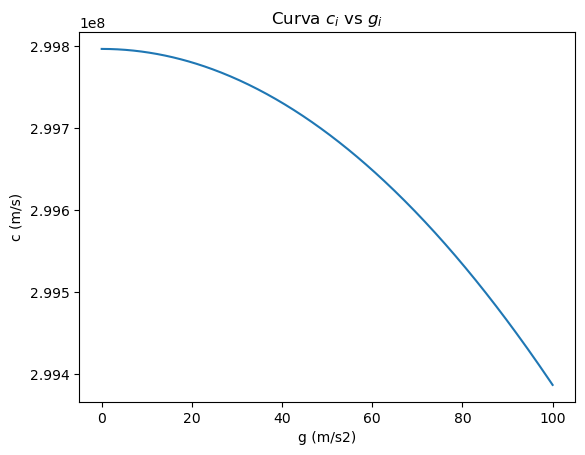
\includegraphics[scale=0.60]{Curva c_i vs g_i.png}
\caption[]{Comportamiento de la ecuación \ref{c_i} como función de $g_i$ en un rango de 0 a 100 m/s$^2$. }
\label{fig:c_itotal}
\end{figure}


\begin{figure}[h]
\begin{center}
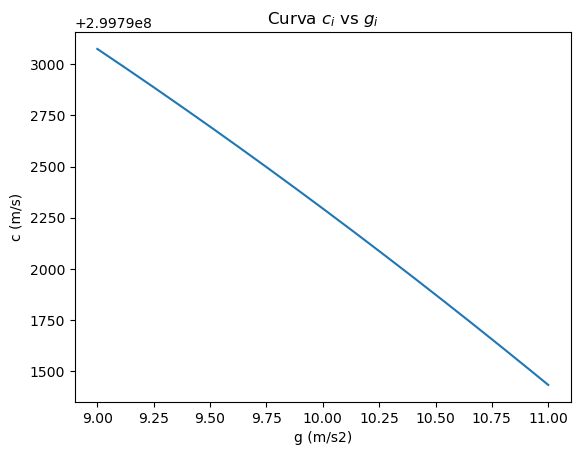
\includegraphics[scale=0.60]{curva c_i vs g_i zoom.png}
\caption[]{Comportamiento de la ecuación \ref{c_i} como función de $g_i$ en un rango de 9 a 11 m/s$^2$. }
\label{fig:c_izoom}
\end{center}
\end{figure}

El resultado de superponer a la línea predicha por la \ac{HCC} los datos proporcionados por Ramdani en la tabla \ref{tab:ramdaniDatos} se tiene en la figura \ref{fig:ramdanisigueHCC}. Se observa que la mayoría de los puntos concuerdan con la predicción dentro de su error, lo cual constituye la última de las justificaciones del presente trabajo.  

\begin{figure}[hbt]
\begin{center}
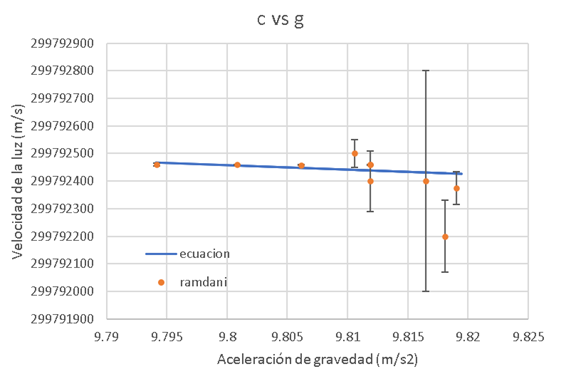
\includegraphics[scale=1]{Imagen4.png}
\caption[]{Datos de velocidad de la luz vs gravedad incluidos en \ref{tab:ramdaniDatos} superpuestos a la linea predicha por \ac{HCC} en la ecuación \ref{c_i}}
\label{fig:ramdanisigueHCC}
\end{center}
\end{figure}


\section{Resultados esperados}

Con el fin de confirmar o refutar la Hipótesis de Céspedes-Curé, se plantea realizar mediciones precisas en tres localidades con diferente valor local de la gravedad, a saber  el campus de la \ac{USB} (Altura 1176 m. Gravedad 977967,685 miligales), en la localidad del teleférico de Caracas (2119 m. 977779,400 miligales) y en la población de Carmen de Urea (Altura  20,36 m. 978251,240 miligales); los valores de la gravedad fueron proporcionados por la Doctora Nuris Orihuela \cite{comunicacionpersonal}. Al aplicar la ecuación \ref{c_i} a cada localidad se tiene que la velocidad de la luz en esos puntos geográficos está dada por los valores incluidos en la tabla \ref{tab:Valores_c_esperados}. Vemos entonces  que los valores de $c$ difieren a partir de la novena cifra significativa, por lo que el mayor reto de la verificación experimental es lograr medidas suficientemente precisas para poder discernir el efecto de la \ac{HCC}.

\begin{table}[h]
\centering
\begin{tabular}{|l|l|l|}
\hline
Localidad & Gravedad m / s² & Velocidad C m / s \\
\hline
Carmen de Urea & 9.7825124 & 29979247\textcolor{blue}{1.69} \\
\hline
USB & 9.77967685 & 29979247\textcolor{blue}{3.97} \\
\hline
Teleférico & 9.777794 & 29979247\textcolor{blue}{5.47} \\
\hline
\end{tabular}
\caption{Valores de gravedad y velocidad de la luz esperada en diferentes localidades, señalando en azul los digitos diferentes entre ellos.}
\label{tab:Valores_c_esperados}
\end{table}


\section{Implicaciones de la HCC}
De demostrarse cierta, la Hipótesis de Céspedes-Curé tendría grandes implicaciones en la física sobre todo en la astronomía, algunas de ellas son:
 \begin{itemize}
     \item \textbf{Explicación a la curva de rotación plana de las galaxias:} Al estudiar como se comporta la velocidad orbital de las estrellas en una galaxia como función de la distancia radial del centro de la misma, se ha encontrado que para una gran parte de los valores más grandes de distancia la velocidad es constante. Para un sistema de este tipo, en el que la mayor cantidad de la masa está en el centro, se espera que la velocidad orbital disminuya con la distancia como pasa, por ejemplo, con los planetas en el sistema solar. Las galaxias tiene mayor masa en su centro, esto se puede saber debido a la gran luminosidad de los mismos debida a la alta densidad de estrellas en esa zona, en comparación con los bordes. Por lo tanto, las velocidades esperadas y las observadas discrepan mucho en su comportamiento, esto ha llevado a interpretar que existe una gran masa distribuida de forma uniforme en las galaxias y la cual no emite luz, la cual se llamó materia oscura. Sin embargo, la \ac{HCC} puede demostrar que la discrepancia de la velocidad se debe, una vez más, a que el efecto Doppler no funciona correctamente por ignorar que la velocidad de la luz es distinta en la región en la que se encuentra la galaxia. De hecho, las estrellas cerca de los bordes experimentan una densidad de energía gravitacional adicional que no perciben las estrellas del centro: la densidad debida a la propia galaxia. Es así como la hipótesis puede solucionar el problema actual de encontrar la materia oscura, simplemente no existe.

\begin{figure}[hbt]
\begin{center}
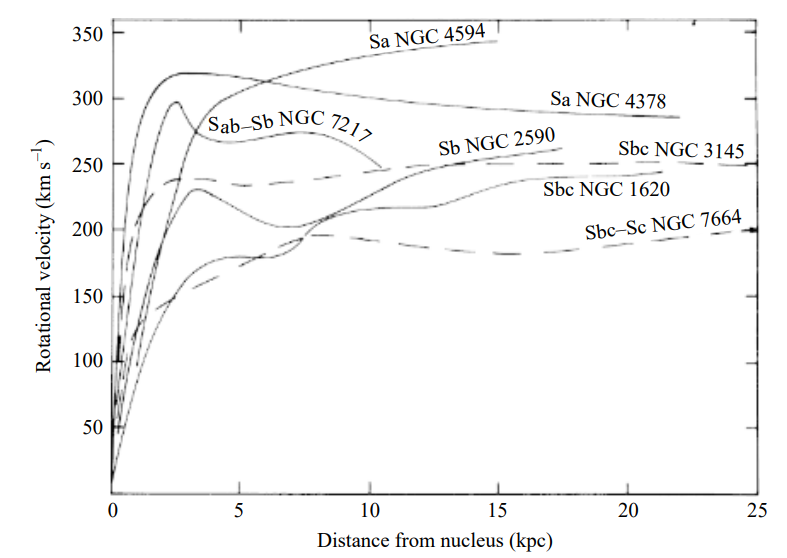
\includegraphics[scale=0.8]{CurvaPlanaGalaxias.png}
\caption[]{Una serie de curvas de rotación para galaxias espirales (figura 24.27 del libro \textit{An introduction to Modern Astrophysics}  \cite{introductiontoastro})}
\label{fig:curvaPlana}
\end{center}
\end{figure}

     \item \textbf{Explicar la expansión acelerada del universo:}  A partir del corrimiento Doppler que muestran las galaxias más lejanas se ha determinado que el universo se expande aceleradamente. Si se asume un universo en expansión con una distribución de masa limitada, la densidad de energía gravitatoria disminuiría hacia los límites, lo que llevaría a un índice de refracción $n'$ cada vez más pequeño y a una velocidad efectiva de la luz $c'$ que aumentaría, resultando en valores sobreestimados de las velocidades de las estrellas deducidas del corrimiento Doppler.

     \item \textbf{Deflexión de la luz de las estrellas por el Sol durante los eclipses solares:} \ac{JCC} en su libro \cite{bib:el-libro} explica este comportamiento de la luz como un fenómeno de refracción causado por el índice de refracción en la vecindad del Sol, que a su vez depende de la densidad de energía gravitacional.

     \item \textbf{Nueva explicación a la existencia de agujeros negros:} Sí se consideran objetos celeste super masivos la densidad de energía gravitacional en su cercanía se hace excesivamente grande, así la \ac{HCC} predice unos valores de velocidad de la luz tan pequeños que percibiríamos el objeto completamente negro \cite{propiedadesdelespaciovacio}.
     
 \end{itemize}

%AL TERMINAR EL CAPITULO PUEDES COMPRAR PAPELERÍA-tres clases del curso de acuarelas



\chapter{Experimento I: Medición directa de la velocidad de la luz}
 
 A continuación se explica el primer experimento realizado, el cual busca medir directamente la velocidad de la luz. Se expone el funcionamiento, el método experimental, el análisis de los datos y los resultados obtenidos; así mismo, se enumeran algunas mejoras realizadas en búsqueda de una mayor precisión. Por último, se calcula la precisión necesaria con este experimento para poder verificar la \ac{HCC} en las localidades planteadas, lo cual explica por qué no es factible el experimento.
 

\section{Introducción}
Para verificar la \ac{HCC} la opción más evidente es la de medir directamente la velocidad de la luz en localidades con diferente densidad de energía, usando los mismos equipos y el mismo método cada vez. Un método sencillo para esto consiste en usar el haz de un láser modulado, el cual se divide haciendo que uno recorra una distancia mucho mayor y variable, y el otro una distancia corta y constante, ambos haces llegan a un mismo sensor donde se estudia el desfase entre ambas señales. El desfase $\Delta t$ aumenta si se aumenta la diferencia de camino $\Delta x$, ya que la relación entre ambos es

\begin{equation} \label{pendiente_c}
    \Delta x = c \Delta t
\end{equation}

de modo que al variar $\Delta x$ se puede trazar una recta cuya pendiente es la velocidad $c$.


\section{Método experimental}

\subsection{Materiales}

\begin{itemize}
    \item Láser de He-Ne
    \item Lente
    \item Espejo con soporte y tornillos de ajuste
    \item Divisor de haz
    \item Generdor de señales moduladas con fotodetectores
    \item Osciloscopio Tektronix TDS 2024B 
\end{itemize}

\subsection{Procedimiento experimental}
Para el montaje experimental se han usado dos variantes. La primera es la usada en la práctica de “Determinación de la velocidad de la luz” en Laboratorio 3 de la \ac{USB} \cite{GUIAlab3}, el esquema se puede ver en la figura \ref{fig:experimento_guia}.


\begin{figure}[hbt]
\centering
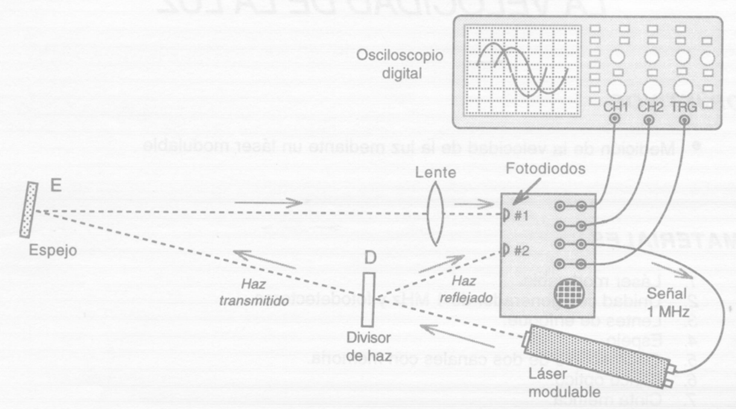
\includegraphics[scale=0.75]{experimento_guia.png}
\caption[]{Esquema experimental para la medición de la velocidad de la luz \cite{GUIAlab3}.}
\label{fig:experimento_guia}
\end{figure}


Se requiere de un láser de He-Ne conectado a un equipo generador de señales moduladas que además tiene incorporados dos fotodetectores, y un osciloscopio en cuyos dos canales se conectaron las señales recibidas por los detectores. La luz del láser pasa por un divisor de haz, el haz reflejado llega a uno de los detectores y el haz transmitido viaja hasta reflejarse en un espejo, y finalmente pasa por un lente que lo enfoca en el otro detector. El espejo se colocó en el extremo opuesto del salón, cada medida tomada se corresponde con una distancia diferente del espejo. Las distancias medidas, usando una cinta métrica convencional, se hicieron directamente de la diferencia de camino entre ambos haces. Para la segunda variante del montaje se reemplazó la señal proveniente del divisor de haz con la misma señal modulada que entra en el láser, mediante una conexión coaxial tipo T, el resto permaneció igual. 

\section{Análisis de datos}
Se usaron dos formas de medir el desfase, una directamente en la pantalla del osciloscopio usando los cursores y mediciones del mismo, y la otra forma extrayendo los datos digitales y haciendo el respectivo análisis. Para las medidas realizadas en la pantalla con los cursores del osciloscopio se ajustaron las dos señales hasta superponerse con amplitudes parecidas y se midió el desfase temporal entre ambas varias veces, tratando de medir siempre la misma parte de la curva. Esta manera de hacerlo permite calcular un promedio que será más fiel al desfase real.

Para la segunda forma, se debe tomar en cuenta que los datos que arroja el osciloscopio utilizado, Tektronix TDS 2024B, vienen en una carpeta de varios archivos, dos .csv cada uno con los valores de las ondas de luz recibidas, una foto de la pantalla del osciloscopio y un archivo .set que no se usó. Para el análisis de los datos (tiempo y voltaje) contenidos en las tablas de los archivos csv es necesario hacer un ajuste sinusoidal de la curva, esto con el fin de identificar las fases de cada una de las señales y poder calcular el desfase entre ellas. 

\begin{figure}[hbt]
\centering
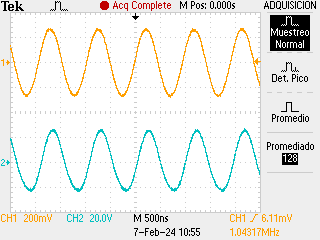
\includegraphics[scale=0.65]{F0003TEK.png}
\caption[]{Ejemplo de imagen de la pantalla del osciloscopio Tektronix TDS 2024B.}
\label{fig:osciloscopio}
\end{figure}

Para hacer el ajuste sinusoidal se creó un programa sencillo con el lenguaje Python. El funcionamiento del programa se basa en 4 etapas, la primera de ellas extrae los datos de tiempo y voltaje del csv. La segunda calcula los parámetros iniciales de búsqueda para el posterior ajuste, donde la frecuencia se calcula usando la Transformada Rápida de Fourier (FFT) de los datos e identificando la frecuencia de mayor amplitud; y la amplitud de la curva usando el cálculo de la desviación estándar. En la tercera etapa se usa la función \textit{curve\_fit}, que al pasarle los parámetros iniciales calculados antes los optimiza para minimizar la diferencia entre los datos de entrada y los valores calculados por la función sinusoidal, a través de métodos de mínimos cuadrados no lineales. Por último, en la cuarta etapa se grafica la curva original junto con la ajustada y se devuelven los parámetros de ajuste. La función de ajuste usada es la siguiente:

\begin{equation}
    A Sin(t \cdot \omega + \phi) + offset
\end{equation}
Por lo que el $\phi$ que arroja el programa está en radianes y debemos transformarlo a tiempo, esto se logra usando
\begin{equation}
    \Delta t = 2 \cdot \frac{|\phi_2 - \phi_1 | }{\omega_2 - \omega_1}
\end{equation}
Donde los subíndices se refieren a cada señal, note que la frecuencia angular usada en esta expresión es un promedio de las dos frecuencias encontradas.


Ya que se aclaró cómo encontrar el desface $\Delta t$ para ambos tipos de medidas realizadas, ahora es necesario calcular la velocidad de la luz. Para ello se usó Excel, donde se grafica $\Delta x$ vs $\Delta t$, recordando que $\Delta x$ es la medida realizada en el laboratorio. Finalmente, usando la formula de pendiente \ref{pendiente_c} se calcula la velocidad de la luz para cada conjunto de medidas. 

\begin{figure}[hbt]
\centering
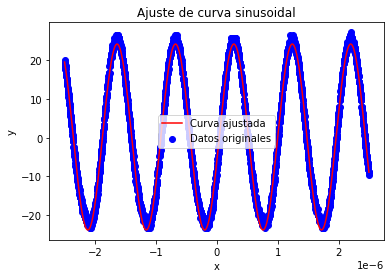
\includegraphics[scale=0.60]{AjusteF0003CH2.png}
\caption[]{Ejemplo de la imagen que devuelve el programa que hace el ajuste de la curva sinusoidal.}
\label{fig:ajusteLaser}
\end{figure}

\section{Resultados}

En cuatro diferentes oportunidades se hicieron mediciones de entre 4 y 7 distancias distintas para probar el montaje, con diferencias de camino entre 10 metros y los 30 metros. Se encontraron resultados poco precisos que se pueden observar en las figuras \ref{fig:C_resultados_malos}, donde todas las gráficas deberían ser una línea recta, y en la tabla \ref{tab:C_resultados_malos} donde se incluyen las pendientes calculadas.


\begin{table}[h]
\centering
\begin{tabular}{|l|l|l|}
\hline
n &  Pendiente (m/s$^2$) \\
\hline
1 & $(3.1666\pm 9.4493)\times 10^8$ \\

2 & $(0.2838\pm0.5678)\times10^8$  \\

3 & $(-0.2135\pm0.2775)\times10^8$\\
4.1 & No aplica \\
4.2 & No aplica \\
\hline
\end{tabular}
\caption{Valores de pendiente y su error para cada medida realizada.}
\label{tab:C_resultados_malos}
\end{table}





\begin{figure}[h!]
    % Primera fila
    \begin{subfigure}[b]{0.5\linewidth}
        \centering
        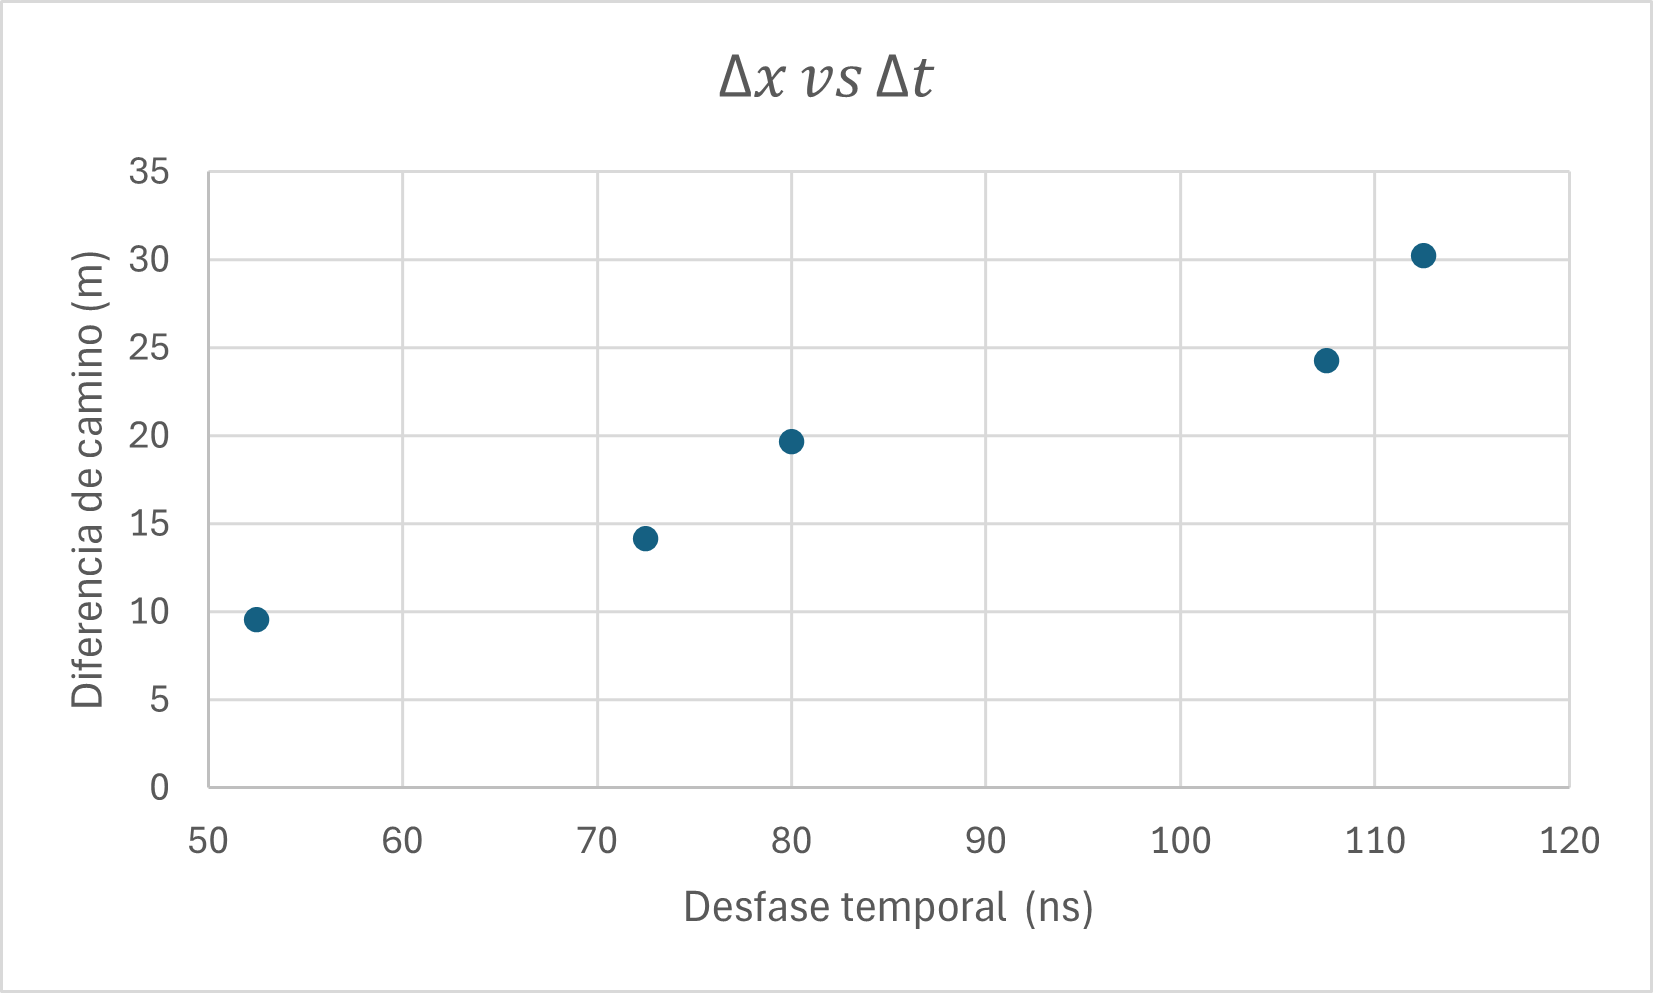
\includegraphics[width=\linewidth]{n-1.png} 
        \caption{Medida n1}
        \label{fig:n1}
    \end{subfigure}
    \hfill
    \begin{subfigure}[b]{0.5\linewidth}
        \centering
        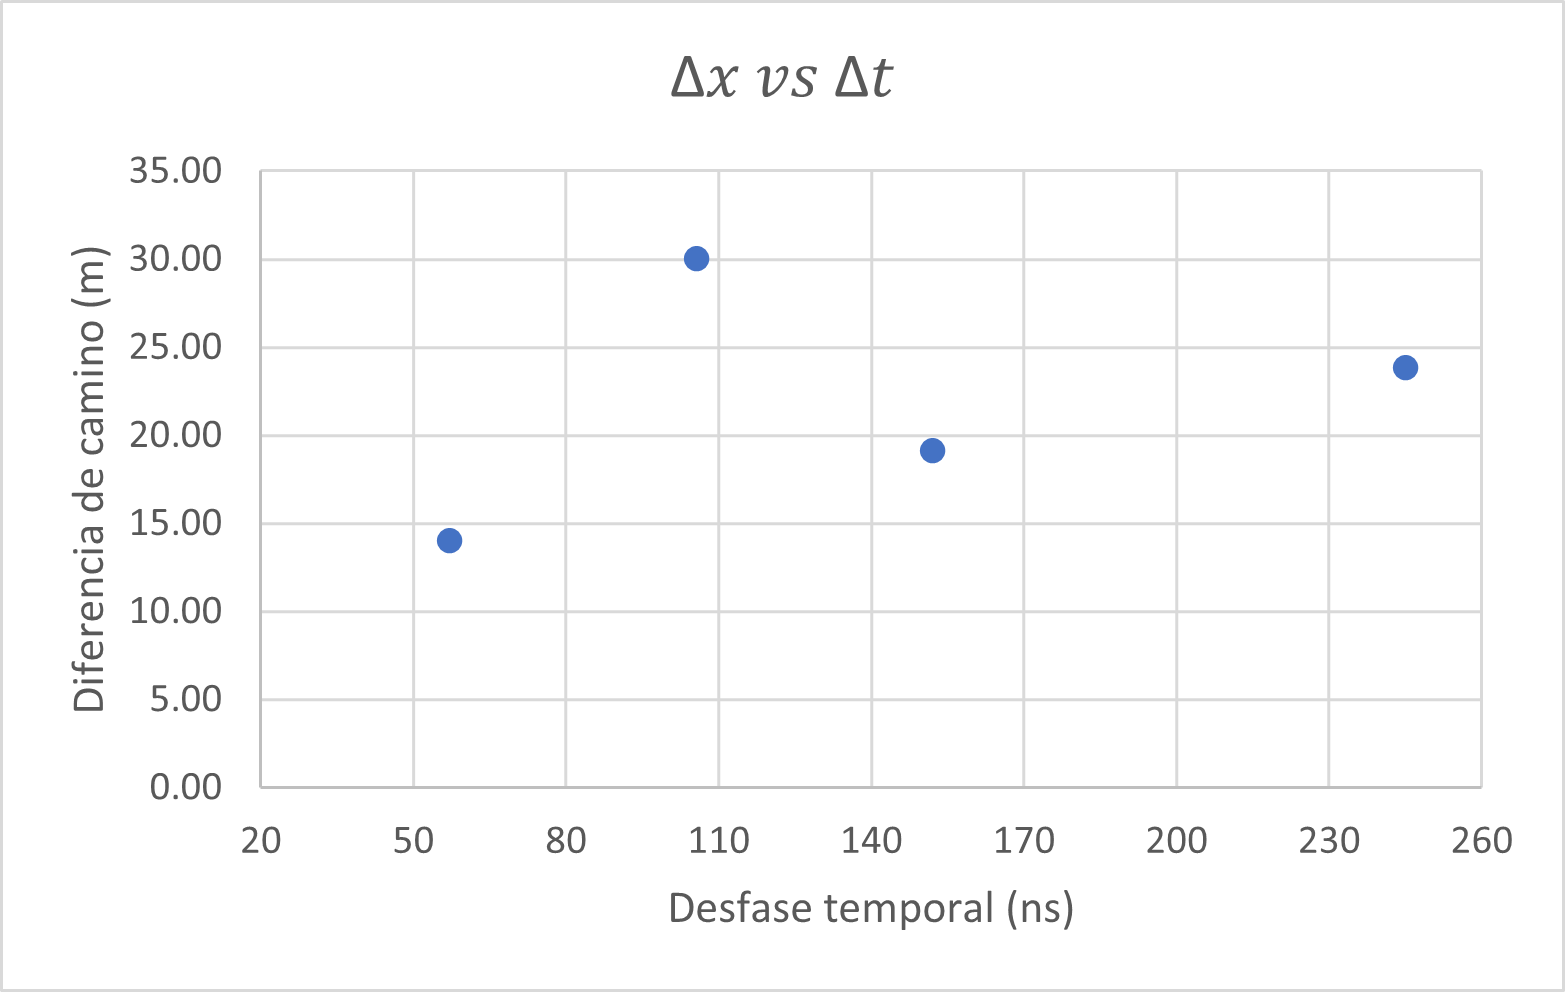
\includegraphics[width=\linewidth]{n-2.png} % Ruta de la segunda imagen
        \caption{Medida n2}
        \label{fig:n2}
    \end{subfigure}

    % Segunda fila
    \vspace{1em}
    \begin{subfigure}[b]{0.5\linewidth}
        \centering
        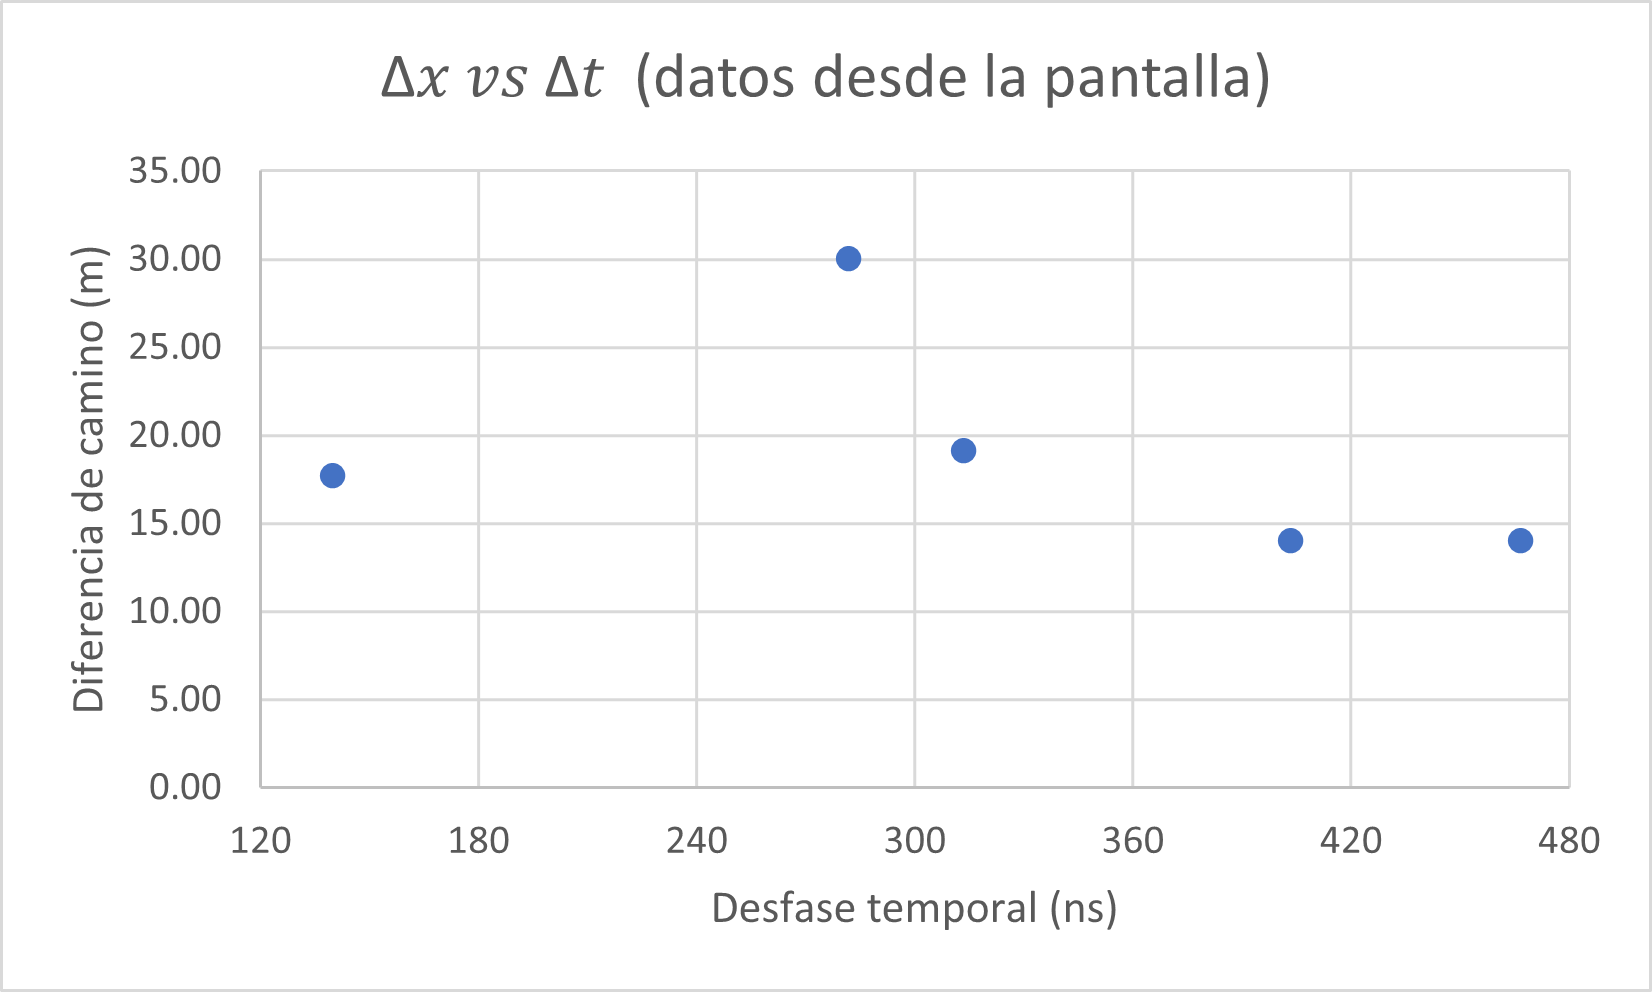
\includegraphics[width=\linewidth]{n-3.png} % Ruta de la tercera imagen
        \caption{Medida n3}
        \label{fig:n3}
    \end{subfigure}
    \hfill
    \begin{subfigure}[b]{0.5\linewidth}
        \centering
        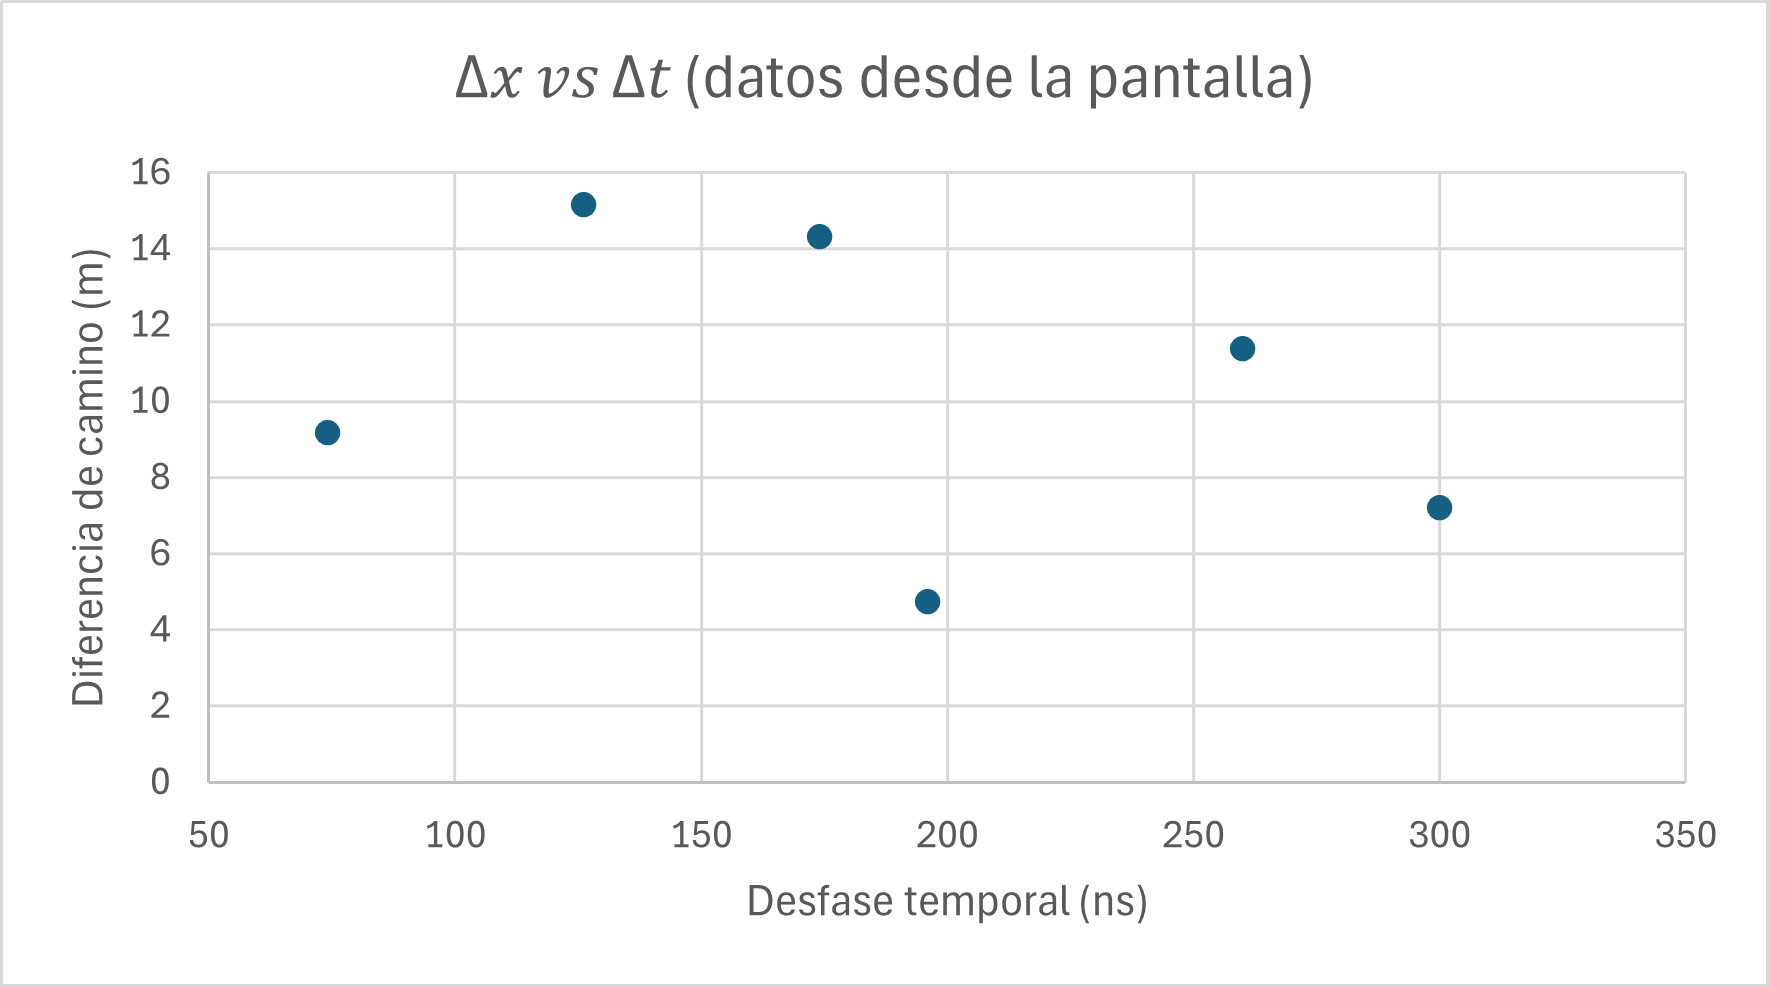
\includegraphics[width=\linewidth]{n-4.1.png} % Ruta de la cuarta imagen
        \caption{Medida n4.1}
        \label{fig:n4.1}
    \end{subfigure}

    % Tercera fila
    \vspace{1em}
    \begin{subfigure}[b]{0.5\linewidth}
        \centering
        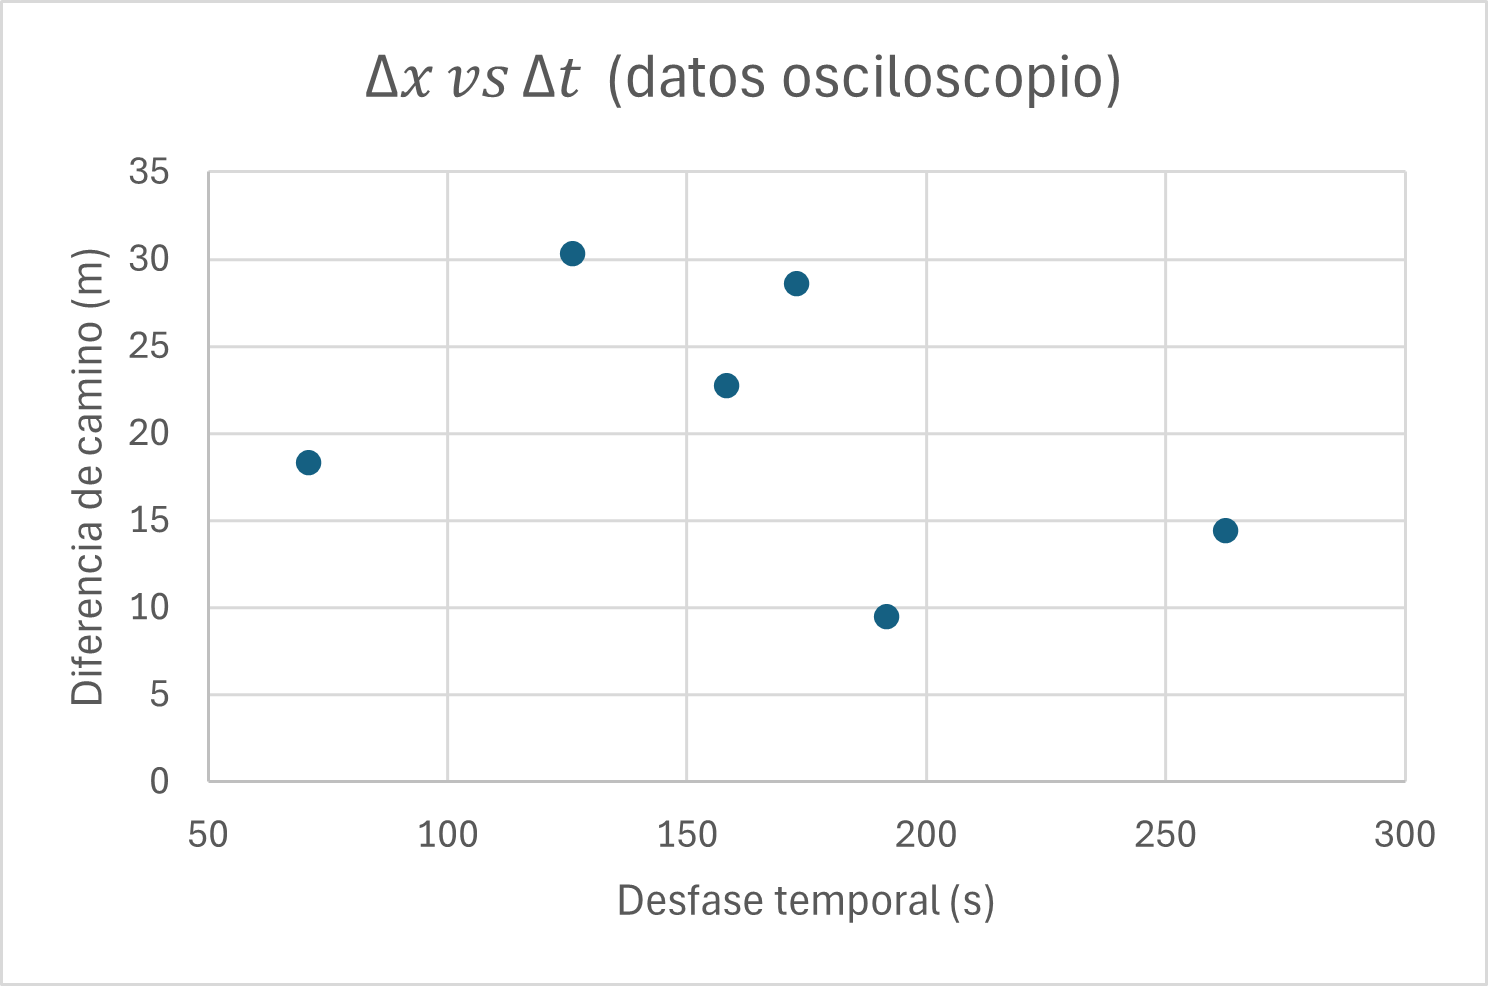
\includegraphics[width=\linewidth]{n-4.2.png} % Ruta de la quinta imagen
        \caption{Medida n4.2}
        \label{fig:n4.2}
    \end{subfigure}

    \caption{Gráfica de los puntos encontrados para cada medida realizada.}
    \label{fig:C_resultados_malos}
\end{figure}

 La medida n1 fué la más cercana al valor esperado de $c$, sin embargo igual cuenta con una gran incertidumbre. Las medidas n2 y n3 tienen pendientes con un orden de magnitud menor al esperado, y en el caso de la n3 la pendiente tiene signo negativo, lo cual carece de sentido. Así mismo carece de sentido los resultado de la medida n4, para la cual se incluyen aquí los resultados obtenidos tanto por la pantalla del osciloscopio como por el tratamiento de los datos digitales, en este último caso los puntos no siguen una tendencia lineal por lo cual no se pueden analizar.
 
En vista de la falta de precisión encontrada con este experimento, se realizaron algunas mejoras al mismo que se detallan en la siguiente sección.

\subsection{Mejoras del método experimental}

\begin{itemize}
    \item Se encontró que mover la lente convergente mínimamente ocasiona un gran desfase en la señal, por lo que se cambió la lente por una con una distancia focal pequeña y se fabricó un soporte fijo para la misma.
    \item Todos los elementos del montaje se colocaron cuidadosamente a la misma altura, esto con el fin de evitar que el haz de luz incidiera en la lente en diferentes ángulos según se acercara el espejo. Esta mejora también evita que existan discrepancias entre la medida hecha con la cinta y la diferencia de camino real entre los haces, dada por el angulo adicional que puedan tener los haces respecto a la horizontal.
    \item Tomar más medidas mejora la estadística y por ende la precisión, de modo que se aumento la cantidad de valores registrados, de 7 puntos a 15.
    \item Para lograr la mejora anterior también se cambió el lugar de la realización del experimento, a partir de ahora sería el pasillo, el cual es más amplio, permitiendo abarcar distancias mucho más grandes para el recorrido del haz.
\end{itemize}

Posterior a las mejoras mencionadas, se realizó la medida 5, cuyas rectas se incluyen en la figura \ref{fig:C_resultados_no_tan_malos} para los datos tomados en pantalla, n5.1, y los obtenidos por el archivo csv, n5.2.  En este caso se nota la mejoría a simple vista, ya que la recta es evidente; los valores de las pendientes se encuentran en la tabla \ref{tab:C_resultados_no_tan_malos}. Para la recta n5.1 el valor encontrado de la velocidad de la luz difiere con el valor aceptado por tan solo $1\%$, mientras que la medida n5.2 se aleja en $6\%$; sin embargo, esta última cuenta con una precisión mayor. Conociendo el experimento, los equipos con los que se cuenta y la precisión que se puede llegar con ellos cabe la pregunta ¿qué precisión se debe alcanzar con este método para lograr verificar la hipótesis de Céspedes-Curé en las tres localidades planteadas?.


\begin{table}[h]
\centering
\begin{tabular}{|l|l|c|}
\hline
n &  Pendiente (m/s$^2$) & Error Porcentual\\
\hline
5.1 & $(3.0296\pm 0.0556)\times 10^8$ & $1\%$ \\

5.2 & $(3.1965\pm0.0355)\times10^8$ & $6\%$ \\

\hline
\end{tabular}
\caption{Valores de pendiente junto al error porcentual con respecto al valor aceptado de $c$, para la medida realizada después de las mejoras al método experimental.}
\label{tab:C_resultados_no_tan_malos}
\end{table}

\begin{figure}[h!]
    % Primera fila
    \begin{subfigure}[b]{0.5\linewidth}
        \centering
        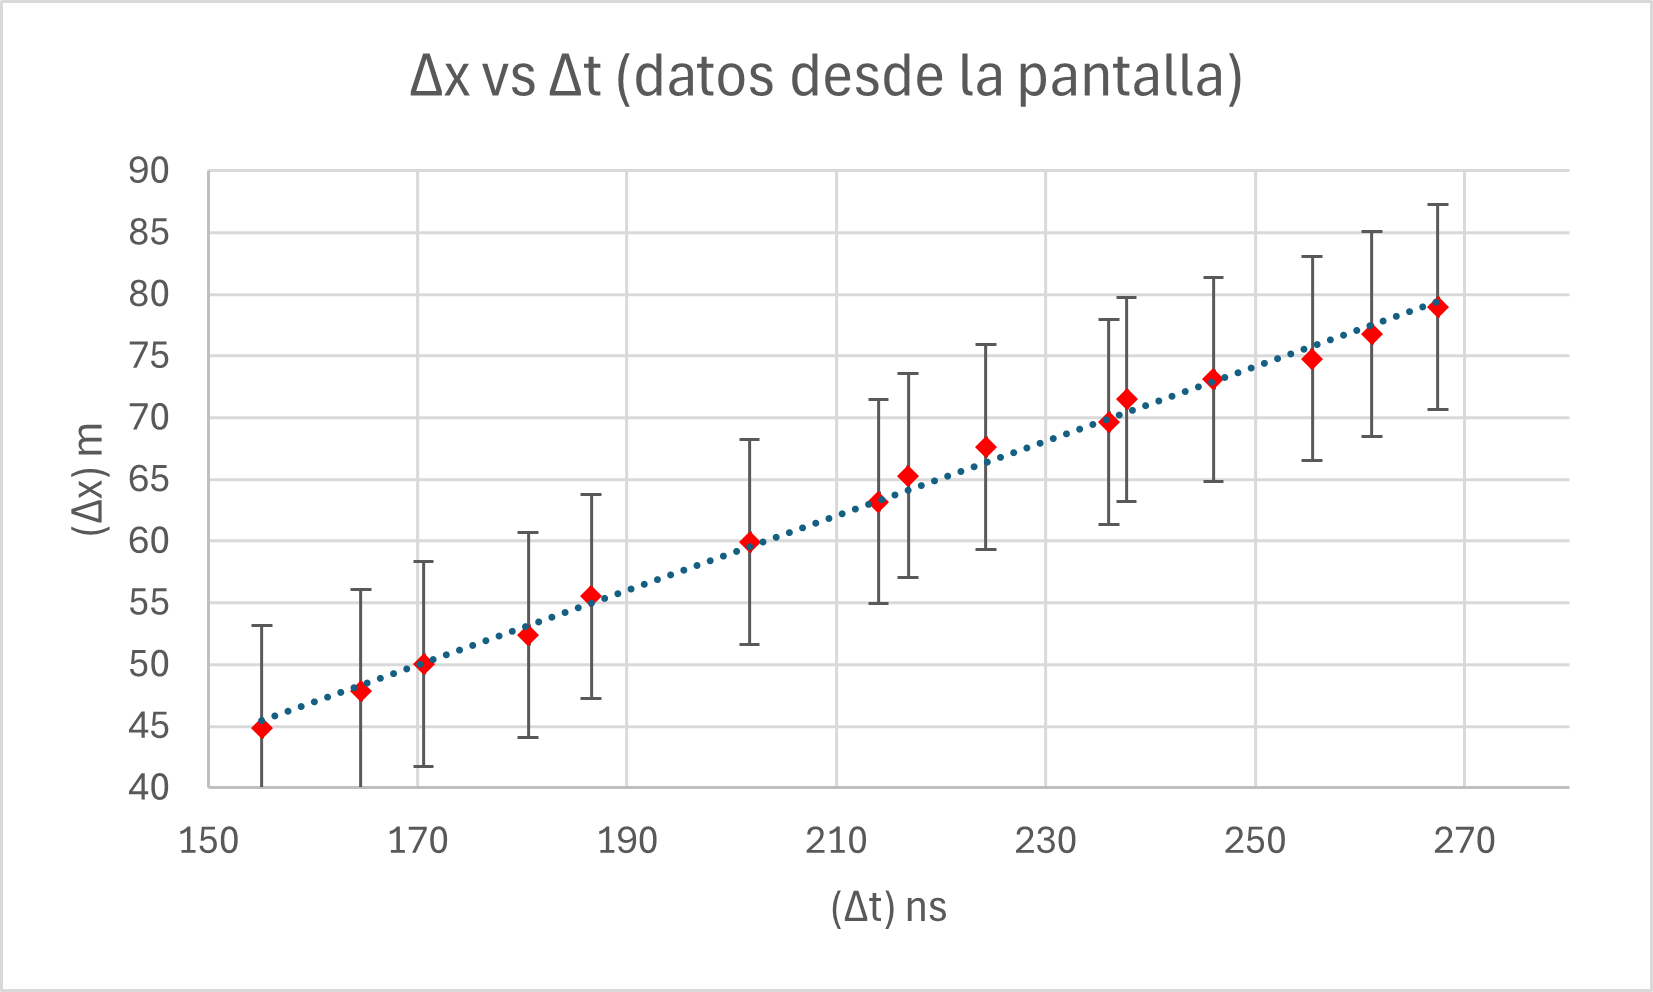
\includegraphics[width=\linewidth]{n-5.1.png} 
        \caption{Medida n5.1}
        \label{fig:n5.1}
    \end{subfigure}
    \hfill
    \begin{subfigure}[b]{0.5\linewidth}
        \centering
        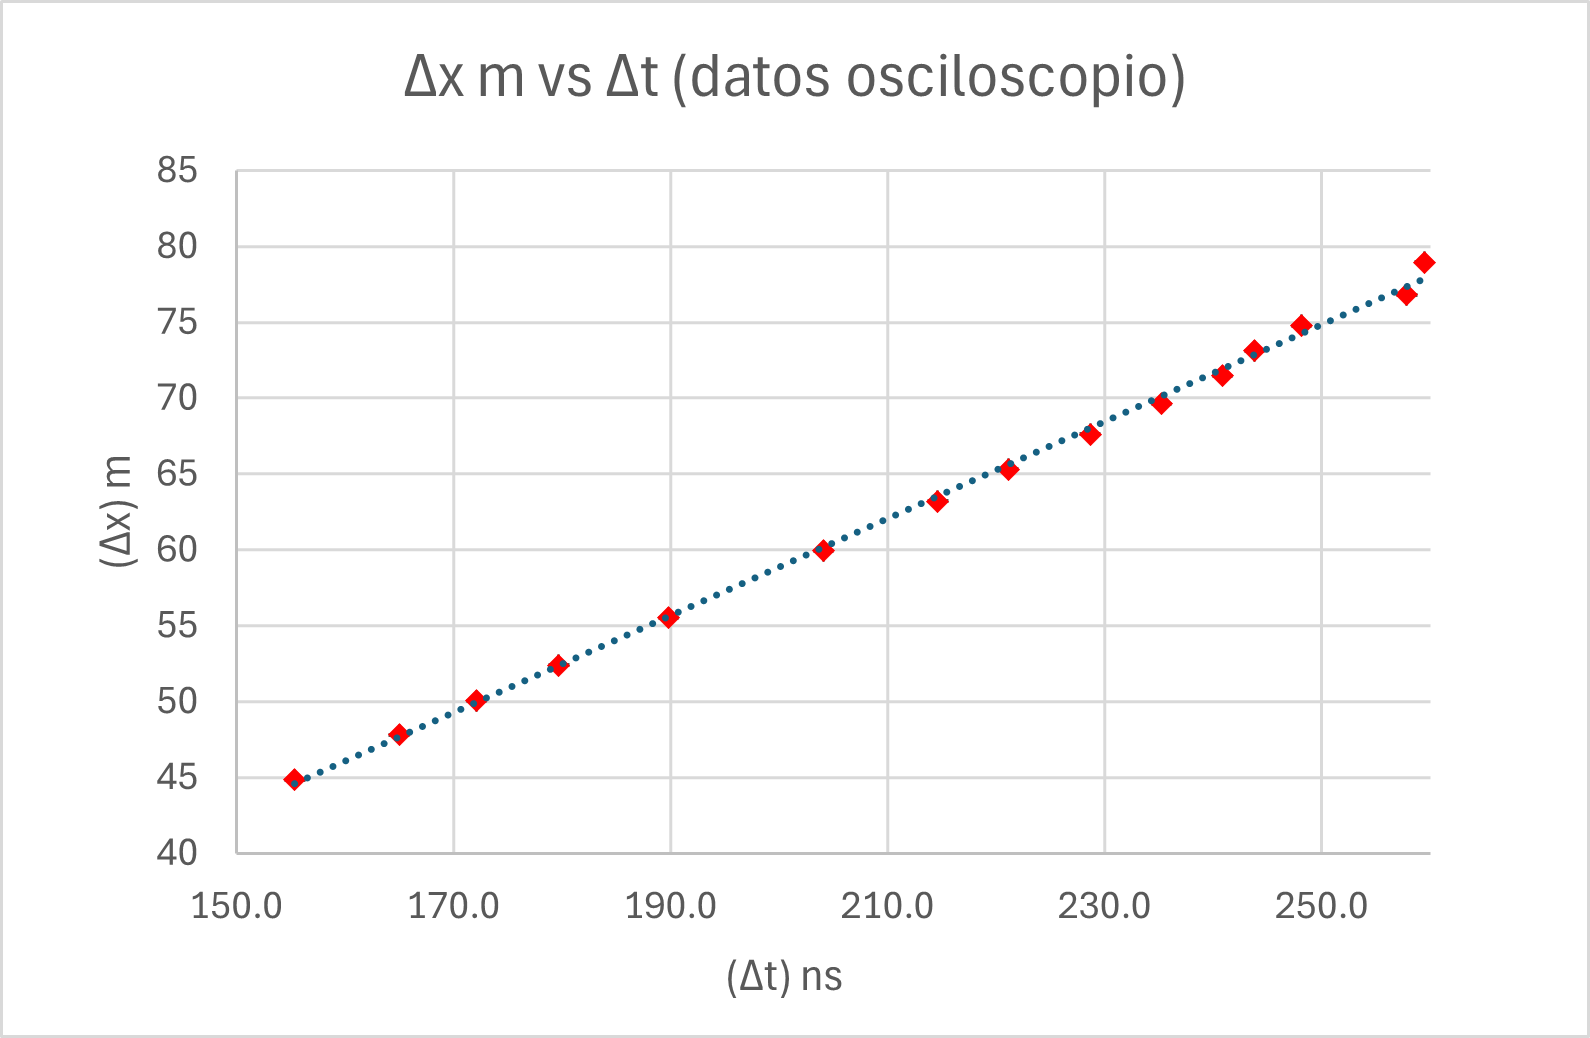
\includegraphics[width=\linewidth]{n-5.2.png} % Ruta de la segunda imagen
        \caption{Medida n5.2}
        \label{fig:n5.2}
    \end{subfigure}
        \caption{Gráfica de los puntos encontrados la mediada realizada despues de aplicar las mejoras, en ambas gráficas se incluyen las barras de error.}
    \label{fig:C_resultados_no_tan_malos}
\end{figure}


\section{Cálculo de la precisión necesaria}


A partir de las velocidades de la luz predichas por la \ac{HCC} para cada localidad, incluidas en la tabla \ref{tab:Valores_c_esperados}, se concluye que el error en las medidas debe ser como máximo de 1 m/s para poder realmente distinguir entre los valores de c y verificar (o no) el cumplimiento de la hipótesis. En este primer experimento para calcular c se usa la siguiente ecuación  
\begin{equation}
    c = \frac{\Delta x}{\Delta t}
\end{equation}
que es la diferencia de camino entre diferencia de tiempo (desfase) entre cada haz de luz que provienen originalmente del mismo láser.  La propagación de errores de dicha ecuación es simplemente

\begin{equation}
    E_c = \frac{E_{\Delta x}}{\Delta t} + \frac{\Delta x}{(\Delta t)^2} E_{\Delta t} 
\end{equation}

Sea $\kappa$ una fracción de la unidad, $0 < \kappa < 1$ , y $F$ otra tal que $F = 1 – \kappa$ entonces podemos dividir el error anterior en sus dos componentes, por una parte

\begin{equation}
    \kappa \cdot E_c = \frac{E_{\Delta x}}{\Delta t} \implies E_{\Delta x} = \kappa \cdot E_c \cdot \Delta t
\end{equation}

y por otra parte

\begin{equation}
    F \cdot E_c = \frac{\Delta x}{(\Delta t)^2} E_{\Delta t} \implies E_{\Delta t} = F \cdot E_c \cdot \frac{(\Delta t)^2}{\Delta x}
\end{equation}

Para estimar los valores de los errores de distancia y tiempo consideremos un error de $c$ de  $E_c = 1$m/s. Para  $\Delta t$ los valores obtenidos están en el orden de los cientos de nano segundos, digamos 200 ns  es decir    $\Delta t= 2 \times 10^{-7}$s y las diferencias de distancias, cuando se hicieron mediciones en el pasillo, estuvieron entre $40$m y $80$m , así que tomemos   $\Delta x= 60$ m como valor representativo. Finalmente, usando los valores detallados anteriormente se tiene que
\begin{align}
    E_{\Delta x} &\sim \kappa \cdot 2 \times 10^{-7} \text{ m} \\
    E_{\Delta t} &\sim F \cdot 6.67 \times 10^{-16} \text{ s}
\end{align}

Entonces, para obtener una velocidad de la luz con una precisión aceptable para diferenciar el efecto de la \ac{HCC} usando este método experimental es necesario que las diferencias de camino sean medidas con una precisión de decenas de nanómetros y las medidas de desfase con precisión de algunos femtosegundos. Es evidente que estas precisiones se escapan de nuestra capacidad. Para la distancia se usa una cinta métrica cuya apreciación es de un milímetro, alcanzar precisiones de nanómetros cuando se miden distancias tan grandes como $80$ m es una tarea complicada. Así mismo ocurre en el caso de la precisión en la medida de desfase, incluso con el osciloscopio y el cálculo de mejor ajuste con Python los errores para los $\Delta t$   están alrededor de $2 \times 10 ^{-10}$ s.

Con el fin de dimensionar y contextualizar la magnitud de la precisión de $c$ que se necesita, consideremos la medición de la velocidad de la luz realizada por Evenson y colaboradores en 1972 \cite{Evenson1972Speed}. En dicho experimento se encontró un valor de c de 299792456.2(1.1) m/s, es decir, una apreciación de la medida parecida a la necesaria para verificar la hipótesis de Cespedes-Curé. El valor encontrado en 1972 es uno de los más precisos y contribuyó a la adopción de la constante de la velocidad de la luz en el vacío como valor definitorio del metro como unidad de distancia. El experimento de Evenson consistía en una medida directa de $c$ pero usando la relación $c=f \lambda$ donde se midió directamente la frecuencia $f$ y la longitud de onda $\lambda$ de la radiación de un láser estabilizado. Para lograr la estabilización del láser y la correcta medición se requieren equipos a los que actualmente no tenemos acceso; por lo tanto, se planteó un nuevo experimento que busca realizar una medición indirecta del efecto de la densidad de energía gravitacional sobre la velocidad de la luz.

\chapter{Experimento II: medición indirecta usando un circuito resonante}

% recuerda incluir que las referencias GuiaLAB-MIT y GuiaLab-SUNY son guias de laboratorio donde se explican este experimento con circuito resonante

%recuerda incluir porque en la suma de las densidades que dice la HCC en este caso importa poco la componente electromagnetica y no es una mala aproximación solo tratar con la parte gravitacional (secreto: esta ultima es muchos ordenes de magnitud (ya eso lo calculó greaves en algun lado) mayor y ademas como el circuito es el mismo la parte electromagnetica más cercana se mantiene) 

AQUI VA EL RESUMEN DEL CAPITULO
\section{Fundamentos teóricos: Electrodinámica y Resonancia}


El objetivo de este planteamiento es el de utilizar la relación de la velocidad de la luz con la permitividad eléctrica $\varepsilon_0$ y la permeabilidad magnética $\mu_0$ dada por
\begin{equation} \label{permitividadyc}
c=\frac{1}{\sqrt{\varepsilon_0\,\mu_0}}
\end{equation}
Donde usaremos el hecho de que $\mu_0$ es una constante cuyo valor es $\mu_0 = 4\pi\cdot 10^{-7}$H/m, por lo que basta con medir la permitividad eléctrica con precisión.

Por otro lado, la capacitancia de un capacitor de placas paralelas está dada por
\begin{equation} \label{capacitanciaplacasparalelas}
C_a=\varepsilon_0\,\frac{A_c}{d}=\frac{1}{c^{2}\mu_0}\,\frac{A_c}{d}
\end{equation}
Con $A_c$ siendo el área de las placas y $d$ la separación entre ellas. En cualquier capacitor se cumple que su capacitancia depende de su geometría y del material, con ecuaciones análogas a \ref{capacitanciaplacasparalelas} en cada caso. Entonces, medir la capacitancia de un capacitor permite conocer el valor de $\epsilon_0$ que es equivalente a medir la velocidad de la luz. 

Una manera de medir indirectamente la capacitancia $C$ es conectar dicho capacitor en serie (o en paralelo) con una resistencia $R$ y un inductor $L$ para crear un circuito R-L-C. La característica principal de este tipo de circuitos es que la energía almacenada en el capacitor se va liberando y a su vez almacenando en el inductor, para ser luego este último el que proporcione la energía al capacitor, en este proceso la corriente eléctrica cambia su dirección de modo que la corriente es alterna. Al aplicarle una corriente de frecuencia $f$ al circuito este responde con la producción de una corriente con la misma frecuencia y distinta amplitud, la amplitud de la corriente será máxima cuando la frecuencia aplicada sea igual a la frecuencia de resonancia del circuito la cual está dada por

\begin{equation} \label{frecuenciaResonancia}
f_0=\frac{1}{2\pi\sqrt{LC}}
\end{equation}

Aquí $L$ es la inductancia de la bobina, entonces si consideramos un solenoide toroidal con núcleo vacío de $N$ vueltas, con área transversal $A_L$ y radio $r$ la inductancia está dada por

\begin{equation}
L=\frac{\mu_0\,N^{2}\,A_L}{2\pi r}
\end{equation}

Como el fin último es medir la velocidad de la luz en diferentes puntos geográficos, si se usa el mismo inductor en el circuito el $L$ no se verá modificado y lo tomamos como una constante. Así al hacer la sustitución de ecuación \ref{capacitanciaplacasparalelas} en \ref{frecuenciaResonancia} nos queda
\begin{equation}
f_0=\frac{c}{2\pi\sqrt{\dfrac{L\,A_c}{d\,\mu_0}}}=k_0\,c
\end{equation}
Donde $k_0$ sería una constante dada por
\begin{equation}
k_0=\frac{1}{2\pi\sqrt{\dfrac{L\,A_c}{d\,\mu_0}}}
\end{equation}
Los valores esperados de $c$ según la hipótesis de Cespedes-Curé para cada uno de los puntos donde se realizarán mediciones ya se expusieron previamente en la tabla \ref{tab:Valores_c_esperados}. Para calcular los cambios esperados en la frecuencia de resonancia del mismo circuito pero en estas tres locaciones tomemos el valor de la constante como $k_0=0.002165397~\text{m}^{-1}$, este cálculo se hace con los siguientes datos $L=6.70\times 10^{-3}\,\text{H}$, $A_c=0.04\,\text{m}^{2}$, $d=0.001\,\text{m}$ y $\mu_0=4\pi\cdot 10^{-7} $ H/m.

\begin{table}[h!]
\centering
\begin{tabular}{lccc}
\toprule
Localidad & Velocidad $C$ m/s & $f_0$ Hz & $f_0/f_{\text{Carmen de Urea}}$\\
\midrule
Carmen de Urea & 299792471.69 & 103318.57\textcolor{red}{0664} & 1\\
USB            & 299792473.97 & 103318.57\textcolor{red}{1449} & 1.000000008\\
Teleférico     & 299792475.47 & 103318.57\textcolor{red}{1966} & 1.000000013\\
\bottomrule
\end{tabular}
\caption{Estimaciones de la frecuencia de resonancia de un circuito RLC según \ac{HCC} en las tres localidades planteadas.}
\end{table}

Se señalan en rojo las cifras que cambian en cada locación. Vemos que para este caso sería necesario alcanzar una resolución de micro Hz para poder apreciar el cambio.


\subsection{Factor de calidad Q}

Es importante señalar que para los circuitos resonantes existe un factor llamado calidad $Q$, el cual mide la eficiencia del circuito, es decir cuán bien el circuito almacena energía en comparación con la energía que pierde. Un alto valor de $Q$ implica una banda de frecuencia estrecha, como para un circuito RLC se tiene que
\begin{equation} \label{factorQ}
Q=\frac{\omega L}{R}
\end{equation}



Basta con disminuir la resistencia y aumentar la inductancia para asegurarnos de tener una función bien estrecha que permita obtener un valor bien preciso de la frecuencia de resonancia.

\begin{figure}[h!]
  \centering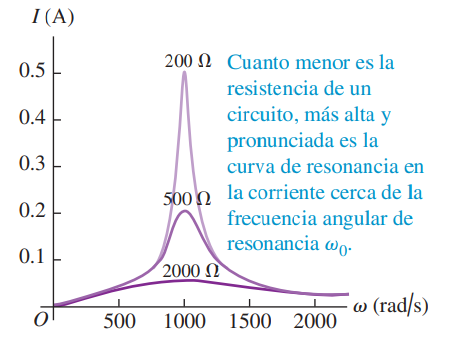
\includegraphics[width=0.6\linewidth]{FactorQ-zemansky.png}\caption{Comportamiento del factor Q según la resistencia en el circuito \cite{searsZemanskyV2}.}
\end{figure}

\section{Planteamiento del procedimiento experimental}

\begin{figure}[h!]\centering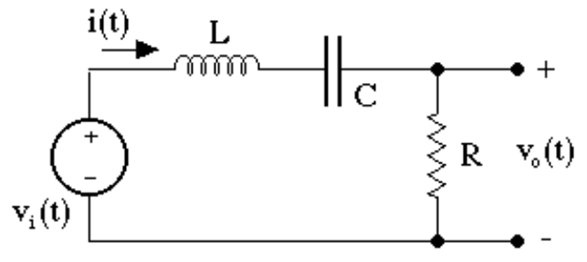
\includegraphics[width=0.5\linewidth]{SUNY-circuito.png}\caption{Circuito RLC en serie planteado por la referencia \cite{GuiaLab-SUNY}.} \label{fig:circuitoGUIASUNY}\end{figure}

Usar la relación \ref{permitividadyc} para estimar el valor de la velocidad de la luz no es algo nuevo \cite{GuiaLab-SUNY}\cite{GuiaLAB-MIT}. Tomemos como punto de partida el montaje experimental plantado en \cite{GuiaLab-SUNY}, donde se usa el esquema de la figura \ref{fig:circuitoGUIASUNY}. Ellos plantean determinar los valores de $L$ y $C$ a partir de las caracteristicas físicas de los componentes electronicos, sin embargo en nuestro caso eso no es necesario ya que el objetivo es comparar el comportamiento del circuito en las tres locaciones, y para ello basta con distinguir el pequeño corrimiento del pico en el barrido de frecuencia que predice la \ac{HCC}.

Un cambio adicional necesario en el montaje experimental es que el mismo se pueda conectar a una computadora, o un Arduino, que permita controlar tanto los cambios de frecuencia de la fuente variable como la amplitud de la corriente en el circuito simultáneamente y de manera automática, esto con el fin de realizar miles de mediciones en un periodo de tiempo corto y para trazar una gráfica exenta de errores humanos.

\subsection{Análisis de la respuesta en serie y simulaciones de sensibilidad}

Supongamos que trabajamos con los mismos valores con los que se calculó la frecuencia de resonancia antes, la amplitud de la corriente en el circuito está dada por
\begin{equation}
I=V/Z
\end{equation}
Donde $Z$ es la impedancia, por lo tanto
\begin{equation}
I=\frac{V}{\sqrt{R^{2}+\left(2\pi f L-\dfrac{1}{2\pi f C}\right)^{2}}}
\end{equation}
Al sustituir la ecuación (2) se tiene
\begin{equation}
I=\frac{V}{\sqrt{R^{2}+\left(2\pi f L-\dfrac{1}{2\pi f}\,\dfrac{c^{2}\mu_0\,d}{A_c}\right)^{2}}}
\end{equation}
Simplificando un poco
\begin{equation}
I=\frac{V}{\sqrt{R^{2}+\left(2\pi f L-\dfrac{2\,c^{2}\,d\cdot 10^{-7}}{f\,A_c}\right)^{2}}}
\end{equation}
A continuación, una gráfica de esta función usando valores de la frecuencia que van en pasos de $0.1\,\mu\text{Hz}$ (30\,000 puntos graficados en total), donde lo único que cambia es la velocidad de la luz $c$ según los valores que se predicen en la hipótesis de Cespedes-Cure, además el valor de la resistencia usado es de $0.0168\,\Omega$, que es equivalente a un cable de cobre de un metro de longitud y sección transversal de 1 mm$^{2}$, y para el voltaje se usó $1\,\text{mV}$.

\begin{figure}[h!]\centering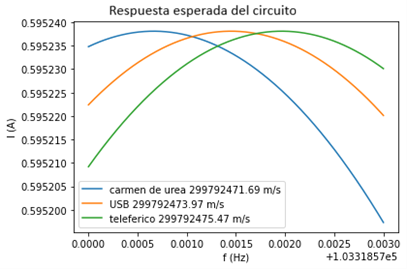
\includegraphics[width=0.90\linewidth]{Simulacion-respuesta1.png}\caption{Curvas $I(f)$ para las tres locaciones.}\label{fig:simulacion1}\end{figure}

En la figura \ref{fig:simulacion2} se puede ver cómo de estrecha es la gráfica en realidad, en este caso se graficaron 10000 puntos igualmente espaciados, ya que con eso es suficiente para darnos una idea de la forma de la función (11) en este caso donde el barrido es entre 103315 Hz y 103322 Hz.

\begin{figure}[h!]\centering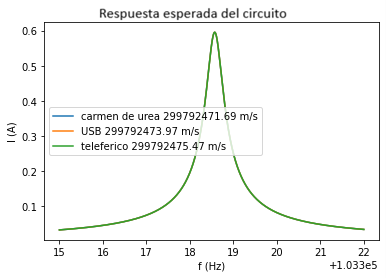
\includegraphics[width=0.90\linewidth]{Simulacion-respuesta2.png}\caption{Detalle de la curva $I(f)$.}\label{fig:simulacion2}\end{figure}

Para que las tres curvas correspondientes a las tres locaciones se puedan identificar correctamente es necesario medir la amplitud de corriente con gran presicion. Si consideramos un multímetro comercial muy preciso conectado en serie dentro del circuito resonante tenemos un problema: las apreciaciones para estos rangos de frecuencias son muy grandes. Es por esto que se obtó por trabajar midiendo la respuesta del voltaje en lugar de la corriente.

%Por ejemplo, para el multímetro más preciso que encontré [4] el rango de 1 A sería perfecto para los valores con los que se está trabajando ya que el error asociado es del orden de 1 $\mu$A, sin embargo, la frecuencia máxima a la que puede realizar mediciones de corriente es 10\,kHz. Disminuir tanto la frecuencia de resonancia de nuestro circuito no es una opción, ya que implica que los cambios en el valor de la frecuencia debido a un cambio en la velocidad de la luz no podrían alcanzarse con la fuente de corriente alterna. Recordemos que dependemos de que la fuente pueda variar con ``pasos'' lo suficientemente pequeños como para alcanzar la frecuencia de resonancia exacta (o por lo menos muy cercana) del circuito en cada uno de los puntos geográficos donde se medirá. Entramos entonces en un ciclo: necesitamos una frecuencia alta para poder medir los cambios de ella (eje $x$ de la gráfica) y necesitamos medir con precisión la corriente (eje $y$) para lo cual se necesita disminuir al menos en dos órdenes de magnitud la frecuencia.Una alternativa pudiera ser el uso de un osciloscopio conectado como lo indica la referencia [2], actualmente estoy trabajando en esa posibilidad\ldots

  


\subsection{Alternativa de medición: Configuración en paralelo}

Otra forma de realizar el circuito es mediante una conexión en paralelo del capacitor y el inductor, como se ve en la figura \ref{fig:RLCparalelosencillo}.

\begin{figure}[h]\centering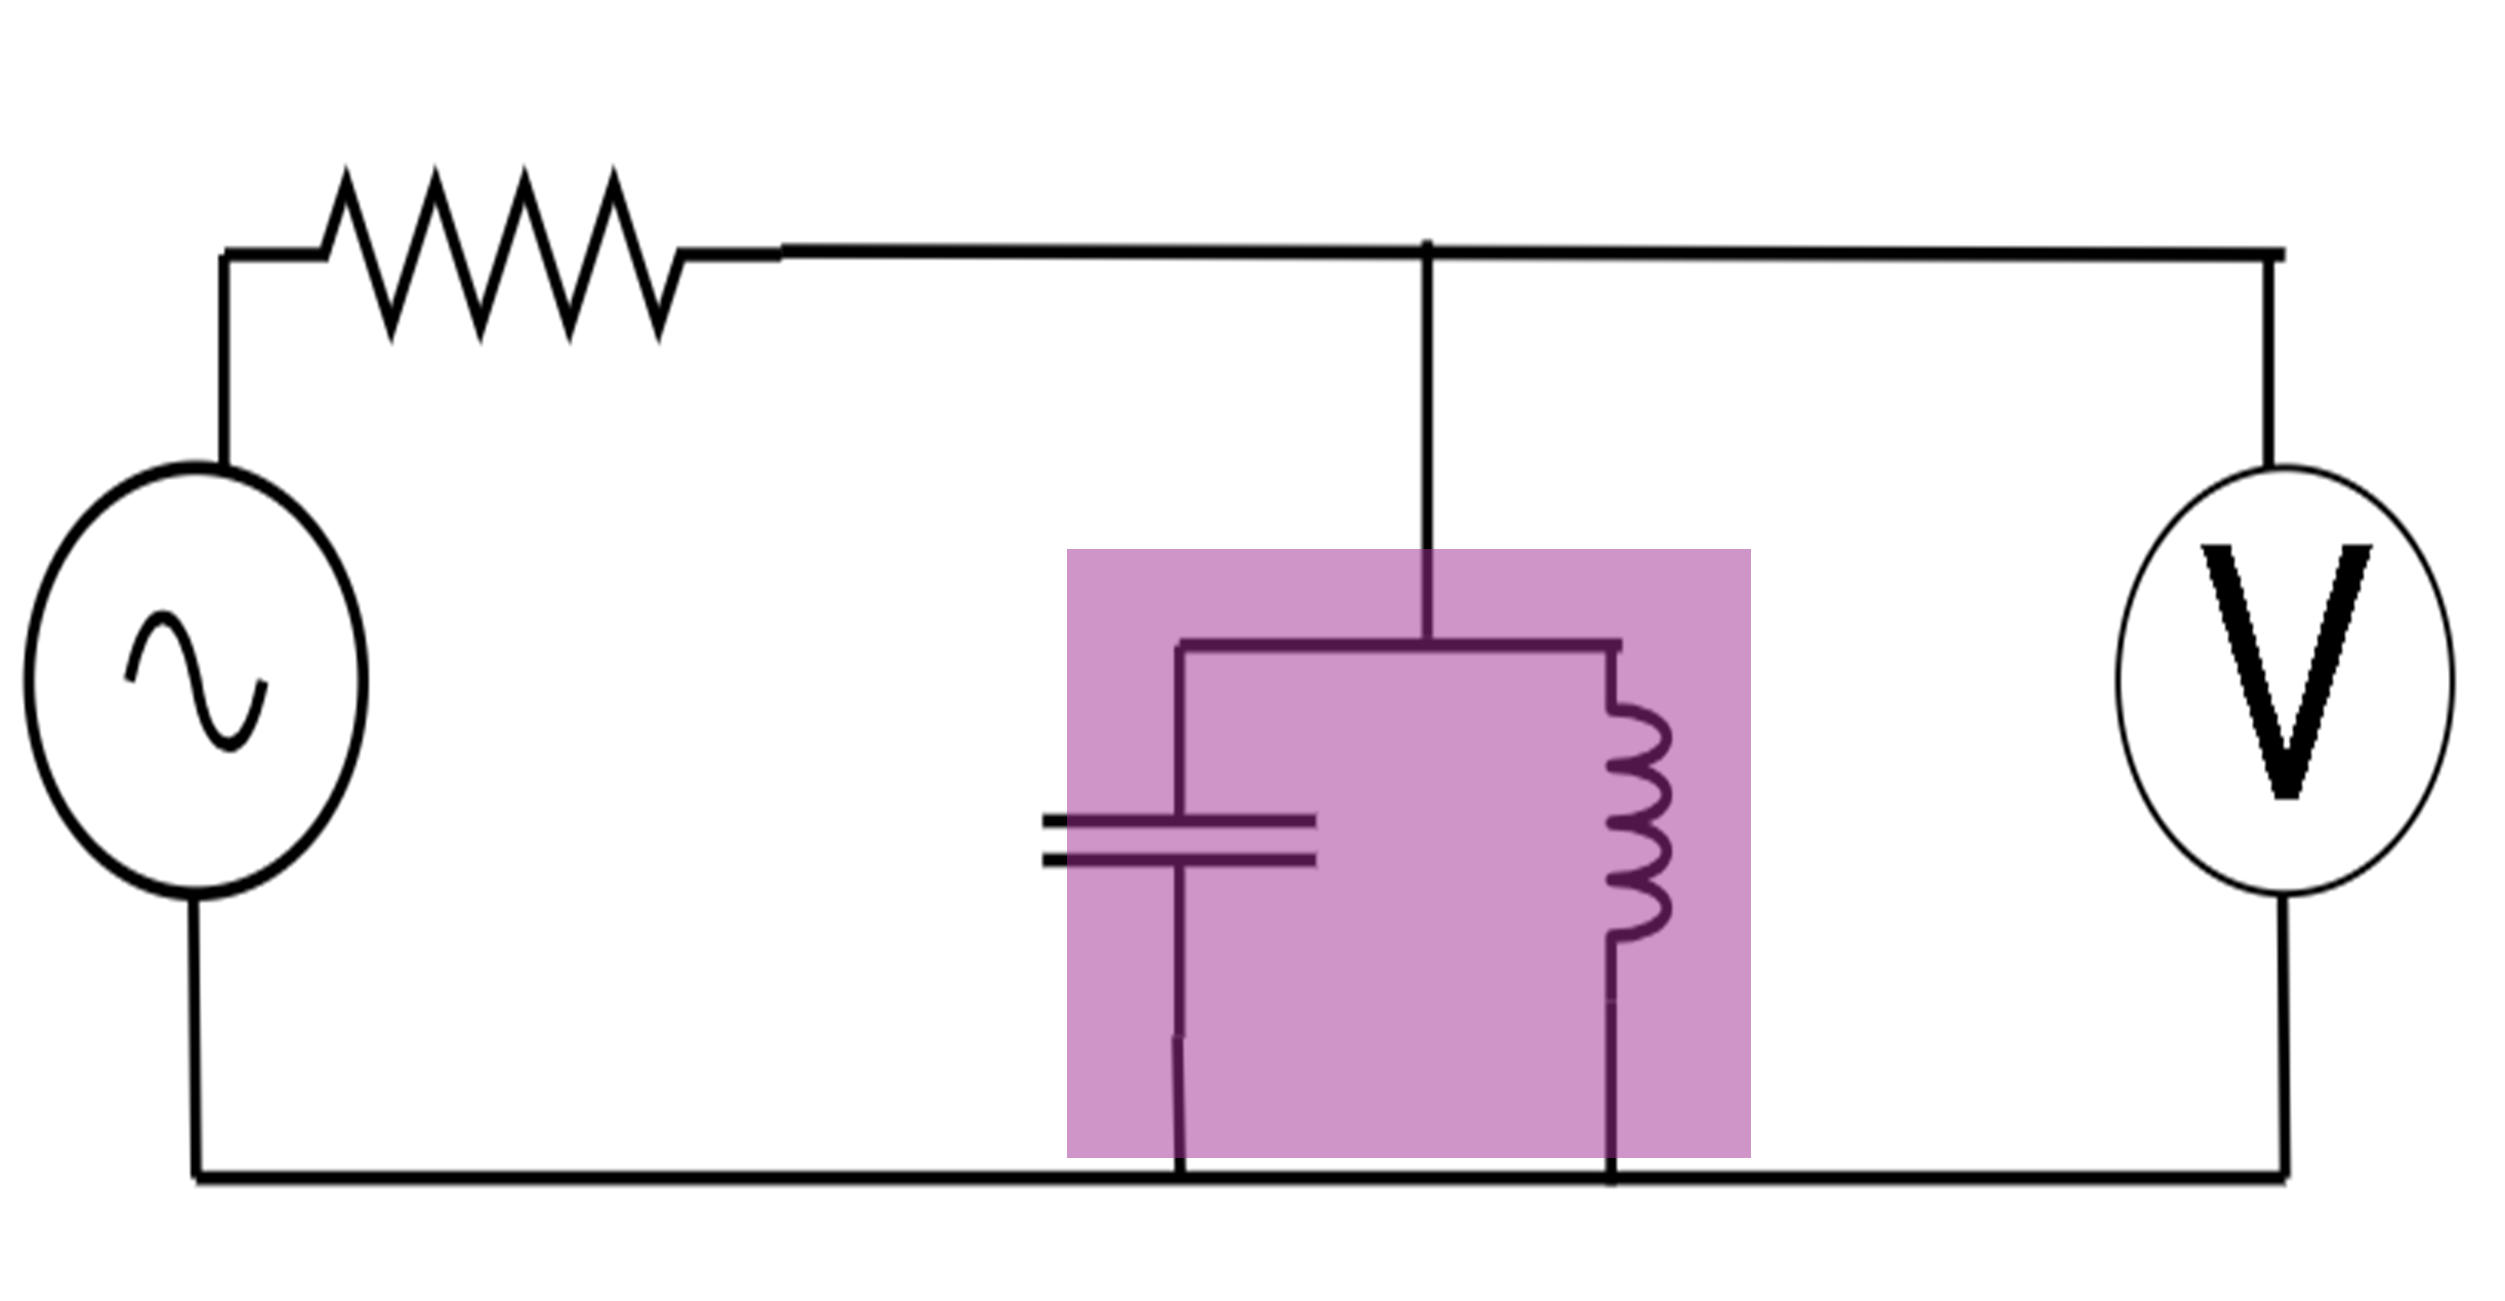
\includegraphics[width=0.45\linewidth]{CL-paralelo-sencillo.png}\caption{Esquema básico de circuito RLC en paralelo.} \label{fig:RLCparalelosencillo}\end{figure}

Es conveniente estudiar cuál será el comportamiento de este circuito planteado. Llamemos $Z_{\text{eq}}$ a la impedancia equivalente del capacitor y el inductor juntos, parte morada en figura \ref{fig:RLCparalelosencillo}. Entonces:
 
\begin{equation}
    \frac{1}{Z_{\text{eq}}} = \frac{1}{Z_C} + \frac{1}{Z_L} = i\omega C + \frac{1}{i\omega L}
\end{equation}
 
\begin{equation}
    Z_{\text{eq}} = \frac{i\omega L}{1 - \omega^2 LC}
\end{equation}
 
Recordando que $V = I\,Z_{\text{eq}}$ y que $\omega = 2\pi f$, como lo que nos interesa es la amplitud del voltaje podemos aplicar el valor absoluto para finalmente tener:
 
\begin{equation} \label{Vparalelo}
    V = \frac{2\pi I f L}{\left|1 - 4\pi^2 f^2 LC\right|}
\end{equation}
 
Esta ecuación tiene valores prácticamente nulos excepto en la frecuencia de resonancia $f_0$, donde tiene asíntota al infinito; sin embargo, es de esperar que al realizar el montaje experimental la amplitud del voltaje a la frecuencia de resonancia no supere el valor de la fuente.
 
Por otro lado, para determinar la amplitud de la corriente $I$ nos ayudamos de la ley de Ohm:
\begin{equation}
    V_1 = IR
\end{equation}
 
donde $V_1$ es la amplitud del voltaje generado por la fuente. Por eso es importante el valor de la resistencia. Finalmente, para poder calcular cuál será el cambio inducido por la hipótesis de Céspedes-Curé es necesario implementar la ecuación \ref{capacitanciaplacasparalelas} en la ecuación \ref{Vparalelo}. Por lo tanto, la amplitud del voltaje viene dada por:
 
\begin{equation}
    V = \frac{2\pi V_1 f L/R}{\left|1 - 4\pi^2 f^2 L \dfrac{1}{c^2\mu_0}\dfrac{A_c}{d}\right|}
\end{equation}
 
Así mismo la frecuencia de resonancia se mantiene como:
 
\begin{equation}
    f_0 = \frac{c}{2\pi}\sqrt{\frac{A_c\,d\,\mu_0}{L}} = k_0 c
\end{equation}
 




\section{????Circuito resonante implementado- esquema experimental}

Para que el experimento pueda funcionar se requiere mucho más que solo una resistencias, un capacitor y una bobina. La propuesta está en añadir modulos adicionales cada uno con su función especifica. El conjunto completo así como las relaciones entre ellos se pueden apreciar en la figura \ref{fig:SOLO-ESQUEMA}

\begin{figure}[hbt]
\begin{center}
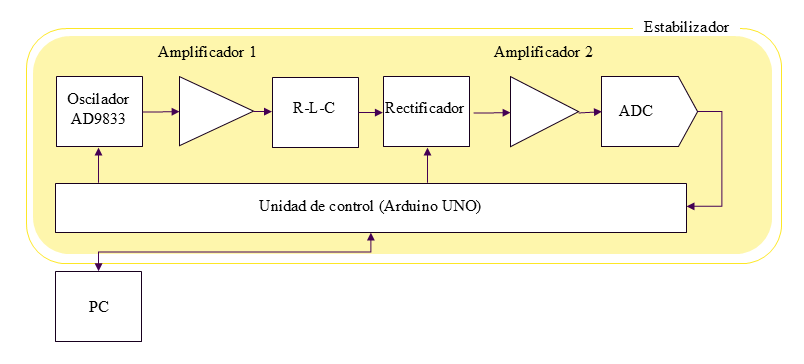
\includegraphics[width=1\linewidth]{SOLO-ESQUEMA.png}
\caption{Modulos del experimento.}
\label{fig:SOLO-ESQUEMA}
\end{center}
\end{figure} 

\subsection{modulo generador}

Se encarga de generar y suministrar la señal sinusoidal al cirucito resonante R-L-C.Se comopone de:
\begin{itemize}
  \item Oscilador AD9833: es un modulo electrónico comercial que permite generar señales muy estables y de INCLUIR CARACTERISTICAS DESTACABLE, REFERRENCIAR AL DATA SHEET
  \item Amplificador 1: Este se encarga de amplificar en voltaje y potencia la señal del generador, esto es necesario para poder excitar el ciruito resonante. INCLUIR LOS DOS CIRCUITOS QUE LO COMPONEN
\end{itemize} 

\subsection{Modulo de lectura}

\begin{itemize}
  \item Rectificador
  \item Amplificador 2 INCLUIR OPAM Y EL DE CANBERRA
  \item ADC INCLUIR SUS CARACTERISTICAS DESTACADAS QUE NOS HICIERON ELEGIRLO, Y REFERENCIAR AL  DATA SHEET
\end{itemize}

\subsection{modulo automatizacion}


\subsection{modulo estabilizador}



\section{Experimento RLC en Serie}
\subsection{procedimiento experimental}
\subsection{Resultados}

\section{Experimento RLC en paralelo}
\subsection{procedimiento experimental}
\subsection{Resultados}



Aquí va el diagrama del circuito y explicación de su funcionamiento
\begin{figure}[hbt]
\begin{center}
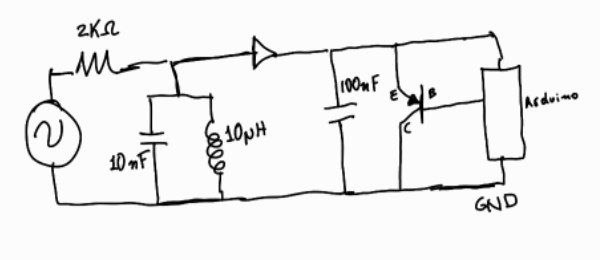
\includegraphics[scale=0.5]{circuitoDibujo.jpg}
\caption[circuito dibujado a mano alzada]{circuito dibujado a mano alzada}
\label{fig:figura1}
\end{center}
\end{figure} 

\begin{figure}[hbt]
\begin{center}
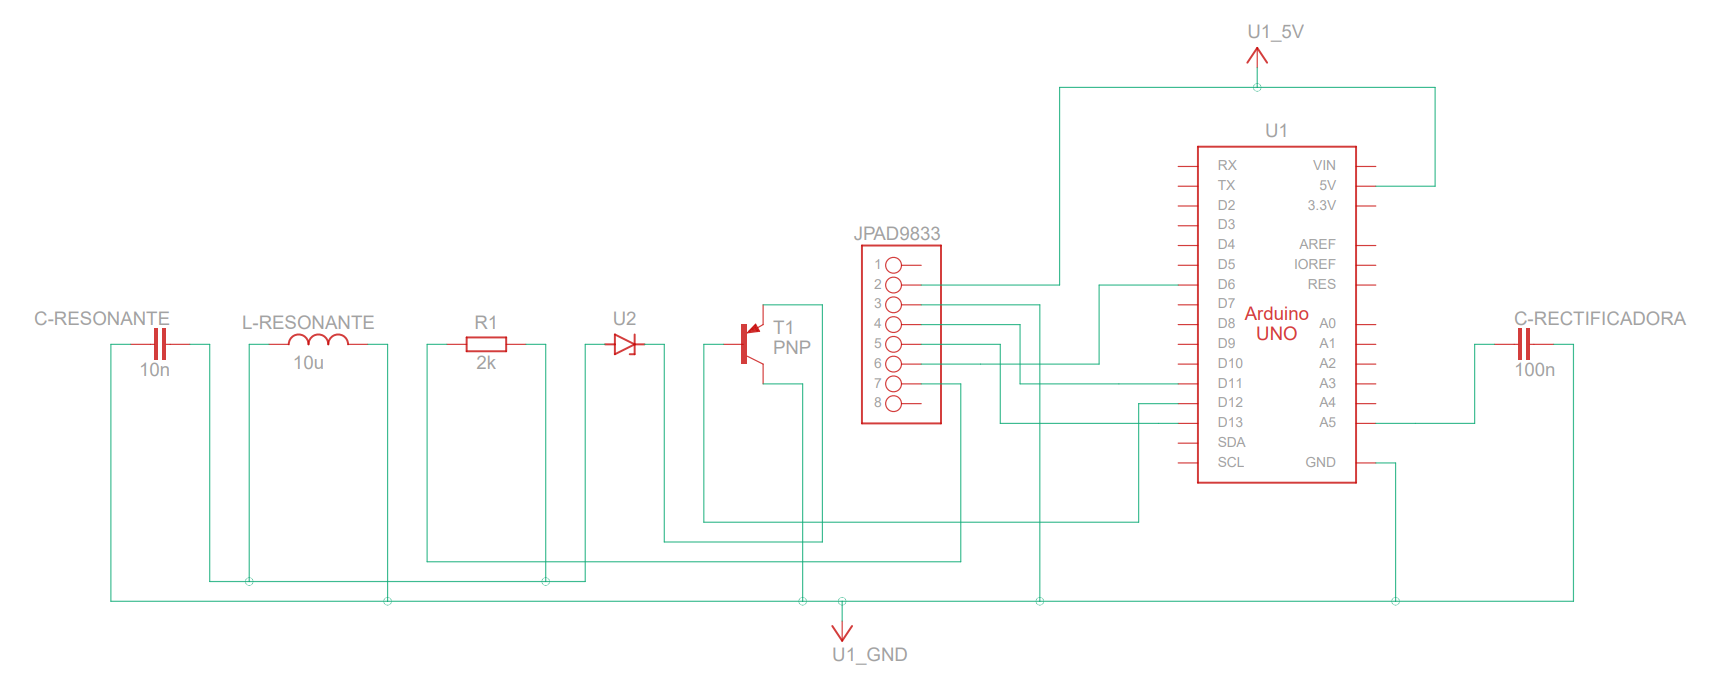
\includegraphics[scale=0.5]{CircuitoCAD.png}
\caption[circuito donde se explica claramente la conexión del arduino,]{circuito donde se explica claramente la conexión del arduino}
\label{fig:figura1}
\end{center}
\end{figure}

Los pines del generador de funciones AD9833 en el diagrama son 
  1-ref
  2-VCC
  3-GND
  4-DAT
  5-CLK
  6-FNC
  7-OUT


\section{Calculo de la precisión necesaria: Ajuste de la curva por ODR}


\section{Modificaciones propuestas} 




hablar sobre la propuesta de prof Julio Wlater
Hablar sobre cambiarse de arduino a red pitaya

\chapter{Experimentos propuestos}
\section{Medición de la velocidad de la luz con gran precisión}
medir la velocidad en distintos puntos con gran precisión (osea la primera idea que teníamos) usando los métodos que en el pasado han dado resultados precisios: ramdani ref 3
\section{Circuito LC en el espacio}
Llevar el equipo descrito en el capitulo III a la estación espacial china.
\section{ Circuito LC con fem aplicada por inducción}

% \begin{figure}[h!]\centering\includegraphics[width=0.6\linewidth]{montaje2.png}\caption{Esquema del segundo montaje.}\end{figure}

En esta segunda forma se conectan la bobina y el condensador en serie, luego se enrolla un cable no aislado alrededor del inductor y los finales de este a un generador de frecuencia, de igual modo se usa otro cable para enrollarlo alrededor del condensador y se conectan sus extremos a un osciloscopio. Este montaje está basado en la referencia \cite{GuiaLAB-MIT}. En este caso la corriente variable $i_0(t)$ induce una fem $\varepsilon$ en el circuito (ley de Faraday) que varía con la misma frecuencia que la corriente original, a su vez $\varepsilon$ genera una corriente inducida $i(t)$ en el circuito LC que tiene la misma frecuencia que $i_0(t)$. Para realizar las mediciones, en la misma referencia [2] se plantea enrollar otro cable no aislado alrededor del inductor (en otra zona del mismo como se ve en la siguiente imagen) y conectar los extremos de este a un osciloscopio.
\chapter*{Conclusiones}

% Para la sección de **Conclusiones**, los lineamientos del Decanato de Estudios Profesionales (DEP) de la USB exigen que estas estén **bien razonadas, fundamentadas y que se deriven de forma lógica** de los resultados obtenidos. 

% Un aspecto normativo crítico que debes cuidar al redactar (y que se observa en los trabajos aprobados de Jesús Ruiz o Celeste Méndez) es que **las conclusiones y las recomendaciones no deben numerarse**. Deben redactarse en forma de prosa fluida, párrafo por párrafo.

% A continuación, te presento un esquema sumamente detallado, estructurado de manera lógica y coherente con el desarrollo experimental de tu tesis, para que te sirva como plantilla de redacción:

% ---

% # ESQUEMA DETALLADO PARA LA REDACCIÓN DE LAS CONCLUSIONES

% ### Parte 1: Conclusión Principal y Viabilidad del Enfoque Indirecto
% *   **Párrafo 1 (La superación del Experimento I y la validez del método RLC):**
%     *   *De qué hablar:* Comienza concluyendo sobre el objetivo principal del trabajo: la viabilidad del método indirecto RLC para registrar variaciones en la velocidad de la luz inducidas por la gravedad, en comparación con el método directo.
%     *   *Qué mencionar:* Contrasta el pobre desempeño del Experimento I (montaje directo con láser y osciloscopio, que solo obtuvo una precisión del 1% y donde el análisis digital a veces no seguía tendencias lineales) con el Experimento II, concluyendo que la vía indirecta a través de la permitividad eléctrica (\\(\epsilon_0\\)) es metodológicamente la única opción viable en el laboratorio para aproximarse a la resolución infinitesimal que exige la verificación de la Hipótesis de Céspedes-Curé (HCC).

% ### Parte 2: Evaluación Técnica del Circuito Resonante
% *   **Párrafo 2 (Configuración Serie vs. Paralelo y Factor de Calidad):**
%     *   *De qué hablar:* Emite un veredicto técnico sobre cuál de las dos configuraciones de circuito resonante evaluadas ofreció un mejor comportamiento físico.
%     *   *Qué mencionar:* Compara los resultados numéricos obtenidos. Explica que, en términos de dispersión y ajuste, los mejores resultados de barrido y estabilidad de la curva se dieron con la **conexión en paralelo** (cuyo error relativo de la frecuencia de resonancia se ubicó en un mínimo de **0.0036%**), mientras que la **conexión en serie** desmejoró notablemente alcanzando un error del **0.34%** (dos órdenes de magnitud por encima).

% ### Parte 3: Desempeño del Control Ambiental e Instrumental
% *   **Párrafo 3 (Estabilización Térmica Activa):**
%     *   *De qué hablar:* Concluye sobre la efectividad del módulo estabilizador autónomo de temperatura y su rol en el control de variables ambientales parásitas.
%     *   *Qué mencionar:* Resalta que el circuito regulador logró mantener la temperatura interna del espacio semiaislado prácticamente constante frente a las fluctuaciones del ambiente exterior. Concluye que esto es un logro indispensable, ya que la aproximación experimental asume que cualquier corrimiento en \\(f_0\\) se debe puramente a la gravedad y no a cambios térmicos que afecten físicamente a los componentes electrónicos.
% *   **Párrafo 4 (La instrumentación y limitaciones del hardware comercial):**
%     *   *De qué hablar:* Analiza críticamente el rendimiento del hardware modular seleccionado (Arduino, oscilador AD9833, convertidor ADS1115).
%     *   *Qué mencionar:* Concluye que la automatización del barrido disminuyó el error humano y permitió registrar curvas suaves, pero el ruido del protoboard, la falta de resistencia de protección en algunos prototipos y la resolución de bits del ADC comercial representaron el principal cuello de botella de hardware para estabilizar la cima de la curva de resonancia.

% ### Parte 4: Rigor Matemático y Análisis DACE (Dispositivos y Algoritmos)
% *   **Párrafo 5 (La superioridad del ajuste ODR sobre el Curve Fit común):**
%     *   *De qué hablar:* Explica la conclusión metodológica fundamental respecto al tratamiento estadístico de los datos.
%     *   *Qué mencionar:* Concluye que, dado que el oscilador AD9833 posee un reloj con un margen de incertidumbre propio (0.1 Hz), el ajuste ordinario de mínimos cuadrados (`curve_fit`) resulta matemáticamente insuficiente porque asume que el eje \\(X\\) no tiene error. Concluye que el uso de la **Regresión Ortogonal de Distancias (ODR)** es obligatorio para ponderar correctamente los errores en ambos ejes, demostrando matemáticamente que la incertidumbre de la frecuencia de resonancia calculada (\\(Var(f_0)\\)) depende tanto de la estrechez de la curva como de la disminución milimétrica del tamaño del paso del barrido.

% ### Parte 5: Alcance Final y Recomendaciones Tecnológicas (Trabajos Futuros)
% *   **Párrafo 6 (El estado actual frente a las tres locaciones propuestas):**
%     *   *De qué hablar:* Sincérate con los resultados finales frente a la meta utópica de medir la variación entre Carmen de Urea, la USB y el Teleférico.
%     *   *Qué mencionar:* Concluye con honestidad científica que los prototipos actuales RLC, aunque estables para barridos macro, aún no alcanzan la resolución de la novena o décima cifra significativa requerida para diferenciar estas altitudes en la Tierra.
% *   **Párrafo 7 (La ruta tecnológica recomendada para el futuro):**
%     *   *De qué hablar:* Plantea soluciones de ingeniería concretas basadas en tus análisis matemáticos finales para las próximas tesis de la USB en esta línea de investigación.
%     *   *Qué mencionar:* Recomienda explícitamente tres mejoras clave estudiadas en tu marco de discusión:
%         1. Implementar la conexión de los módulos resonantes **por inducción** para eliminar la pérdida de energía por cables físicos y simplificar el circuito amplificador.
%         2. Sustituir el Arduino por la plataforma **Red Pitaya STEMlab 125-14** para realizar un muestreo de alta frecuencia y ajustar directamente la señal sinusoidal sin necesidad de rectificación de voltaje.
%         3. Evaluar el comportamiento del transductor mediante la respuesta a un **único pulso de excitación** (señal amortiguada) en lugar del barrido de frecuencia clásico.

% ---

%\nocite{*}
\bibliography{referencias}
\appendix
\chapter{Código Arduino}\label{apx:Arduino}

El programa cargado en el Arduino UNO cumple tres funciones principales: generar la señal sinusoidal de barrido a través del módulo AD9833, adquirir la respuesta del circuito resonante mediante el convertidor analógico-digital ADS1115, y transmitir los datos de frecuencia y voltaje a la computadora por el puerto serial. El ciclo se repite tantas veces como la PC lo indique enviando los parámetros de un nuevo barrido.

\section{Librerías y configuración de pines}

Se emplean cuatro librerías externas: \texttt{SPI.h} y \texttt{MD\_AD9833.h} para controlar el generador de funciones AD9833 por SPI de software, y \texttt{Wire.h} junto con \texttt{Adafruit\_ADS1X15.h} para comunicarse con el ADS1115 por el protocolo de comunicación I$^2$C (\textit{Inter-Integrated Circuit}).

Los pines 13, 12 y 11 están asignados a las líneas de datos, reloj y habilitación del AD9833 respectivamente. El pin digital 9 controla la base del transistor PNP que descarga el capacitor del módulo de lectura; al ser de tipo PNP, una señal \texttt{HIGH} mantiene el transistor apagado y una señal \texttt{LOW} lo enciende.

Las características del barrido quedan definidas por tres variables de punto flotante: la frecuencia de inicio \texttt{f}, la frecuencia final \texttt{f\_final} y el incremento entre pasos \texttt{f\_inc}. Estos valores no están fijados en el código sino que son enviados por la PC antes de cada barrido, lo que permite modificar el rango y la resolución sin reprogramar el Arduino.

\section{Inicialización}

La función \texttt{setup()} inicializa la comunicación serial a 115200 baudios, el módulo AD9833 (incluyendo un reset para asegurar un estado conocido), y el ADS1115 con una ganancia de \texttt{GAIN\_EIGHT} ($\pm\,0.512\,$V, resolución de $0.015625\,$mV/bit), elegida para adecuar el rango del ADC al nivel de voltaje esperado a la salida del módulo de lectura. El transistor se deja inicialmente apagado y se envía el mensaje \texttt{Arduino listo} por serial para confirmar a la PC que el sistema está operativo.

\section{Ciclo principal}

La función \texttt{loop()} opera en dos bloques. En el primero, si hay datos disponibles en el puerto serial, se leen los tres parámetros del barrido separados por comas y terminados en salto de línea (\texttt{f}, \texttt{f\_final}, \texttt{f\_inc}), y se activa la bandera \texttt{procesandoDatos}.

En el segundo bloque, activo mientras \texttt{procesandoDatos} sea verdadero y \texttt{f\,<\,f\_final}, se ejecuta el siguiente ciclo para cada punto del barrido:

\begin{enumerate}
    \item Se configura el AD9833 para generar la frecuencia \texttt{f} y se espera 100\,ms para que la señal en el circuito se estabilice.
    \item Se realiza una lectura en el canal 2 del ADS1115 y se convierte a voltios con \texttt{computeVolts}.
    \item Se transmite por serial una línea con el formato \texttt{f,voltaje}, con cuatro y seis cifras decimales respectivamente.
    \item Se enciende el transistor durante 100\,ms para descargar el capacitor del rectificador y luego se apaga, asegurando que cada punto del barrido sea una medición independiente.
    \item Se incrementa \texttt{f} en \texttt{f\_inc} y se espera 50\,ms antes de la siguiente iteración.
\end{enumerate}

Al alcanzar \texttt{f\_final}, la bandera se desactiva y el programa queda a la espera de un nuevo conjunto de parámetros por parte de la PC.
\chapter{Tratamiento de los datos con Python}\label{apx:PC}

INCLUIR EXPLICACIÓN DEL SOFTWARE: EL PYTHON QUE CONTROLA PERO TAMBIEN LA PARTE QUE AJUSTA LA CURVA

\begin{figure}[ht]
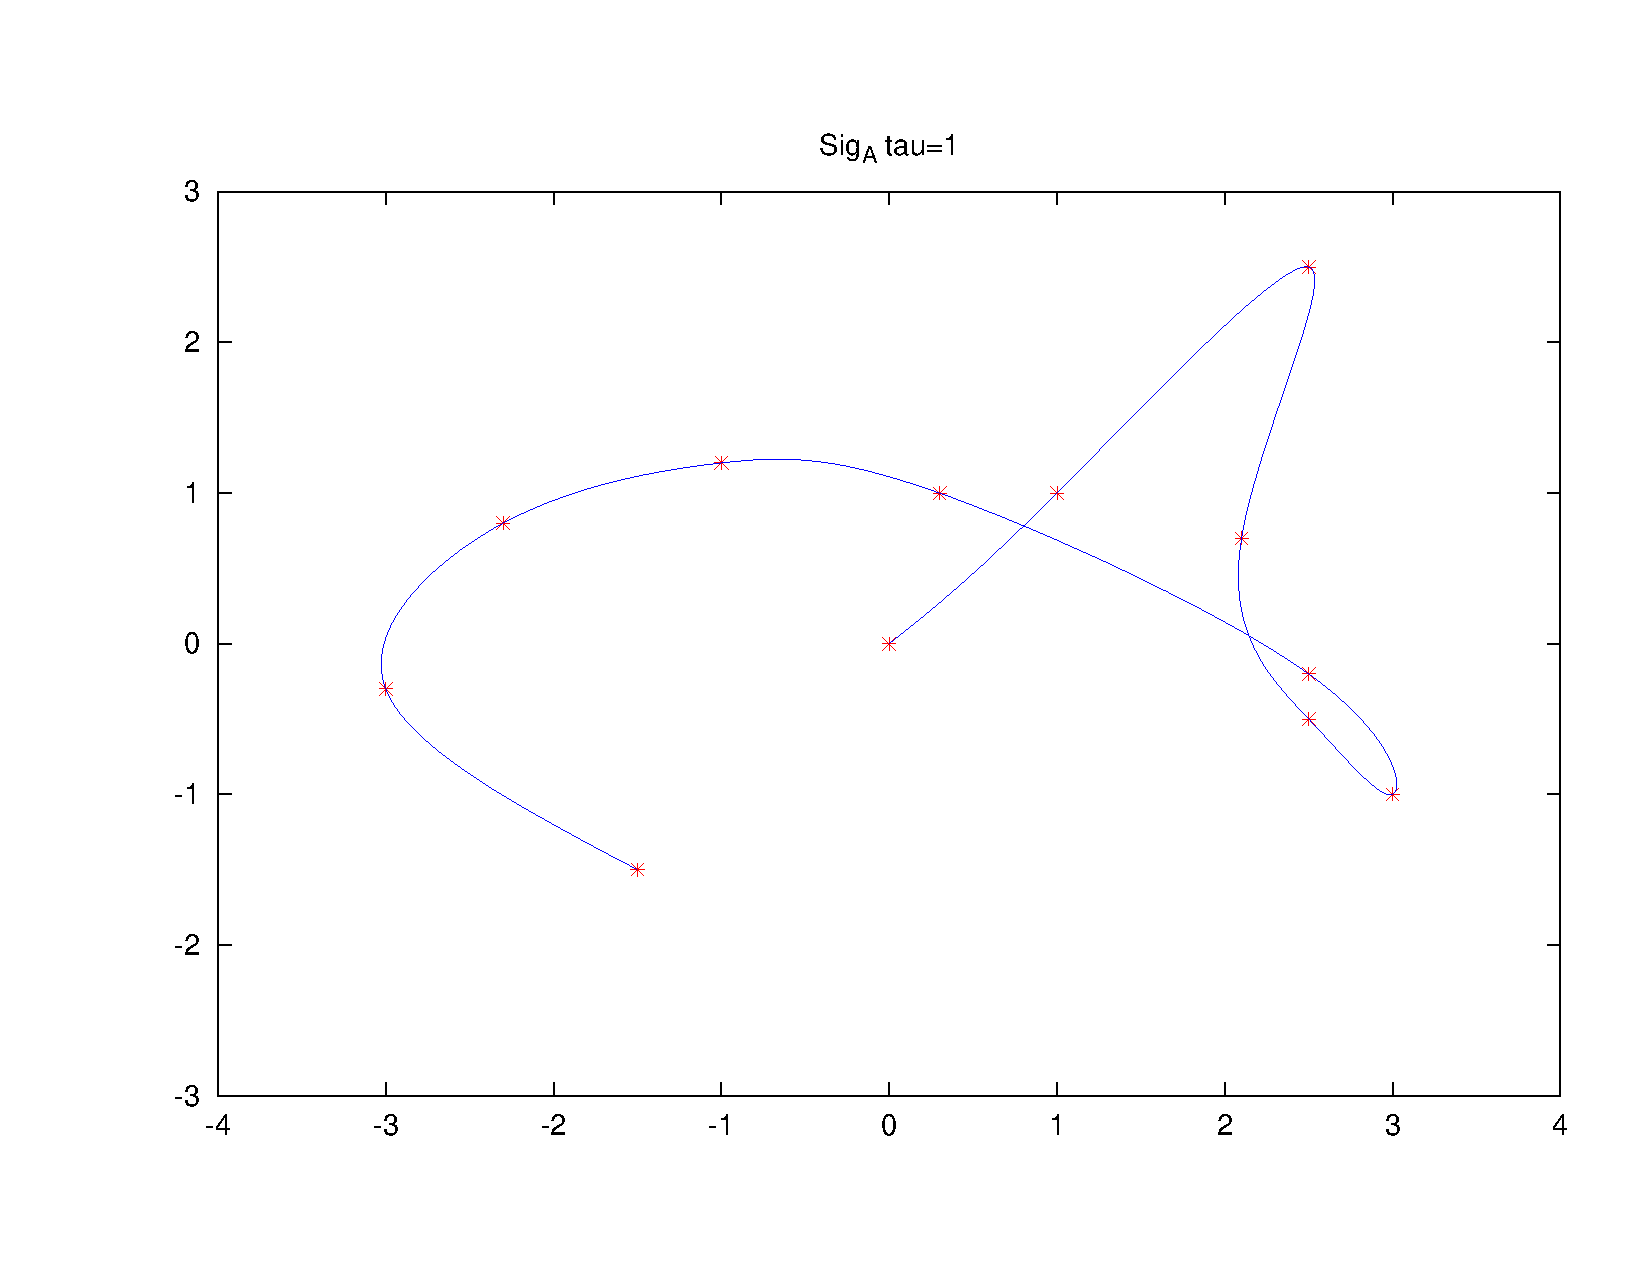
\includegraphics[scale=0.48,angle=0]{ejemplo}
\caption[Título corto de imagen]{Título corto de imagen}\label{img:imgscl}
\end{figure}



\chapter{Apéndice C: Esquemático completo del circuito resonante en serie} % Título centrado y en negrita según norma
\addcontentsline{toc}{chapter}{Apéndice C: Esquemático del circuito}
\label{ape:esquematico}

% Usamos sidewaysfigure para que el esquema se vea en horizontal y sea legible
\begin{sidewaysfigure}[htbp]
    \centering
    % Ajusta el width al 1.0 para que use todo el ancho de la página tabloide/carta
    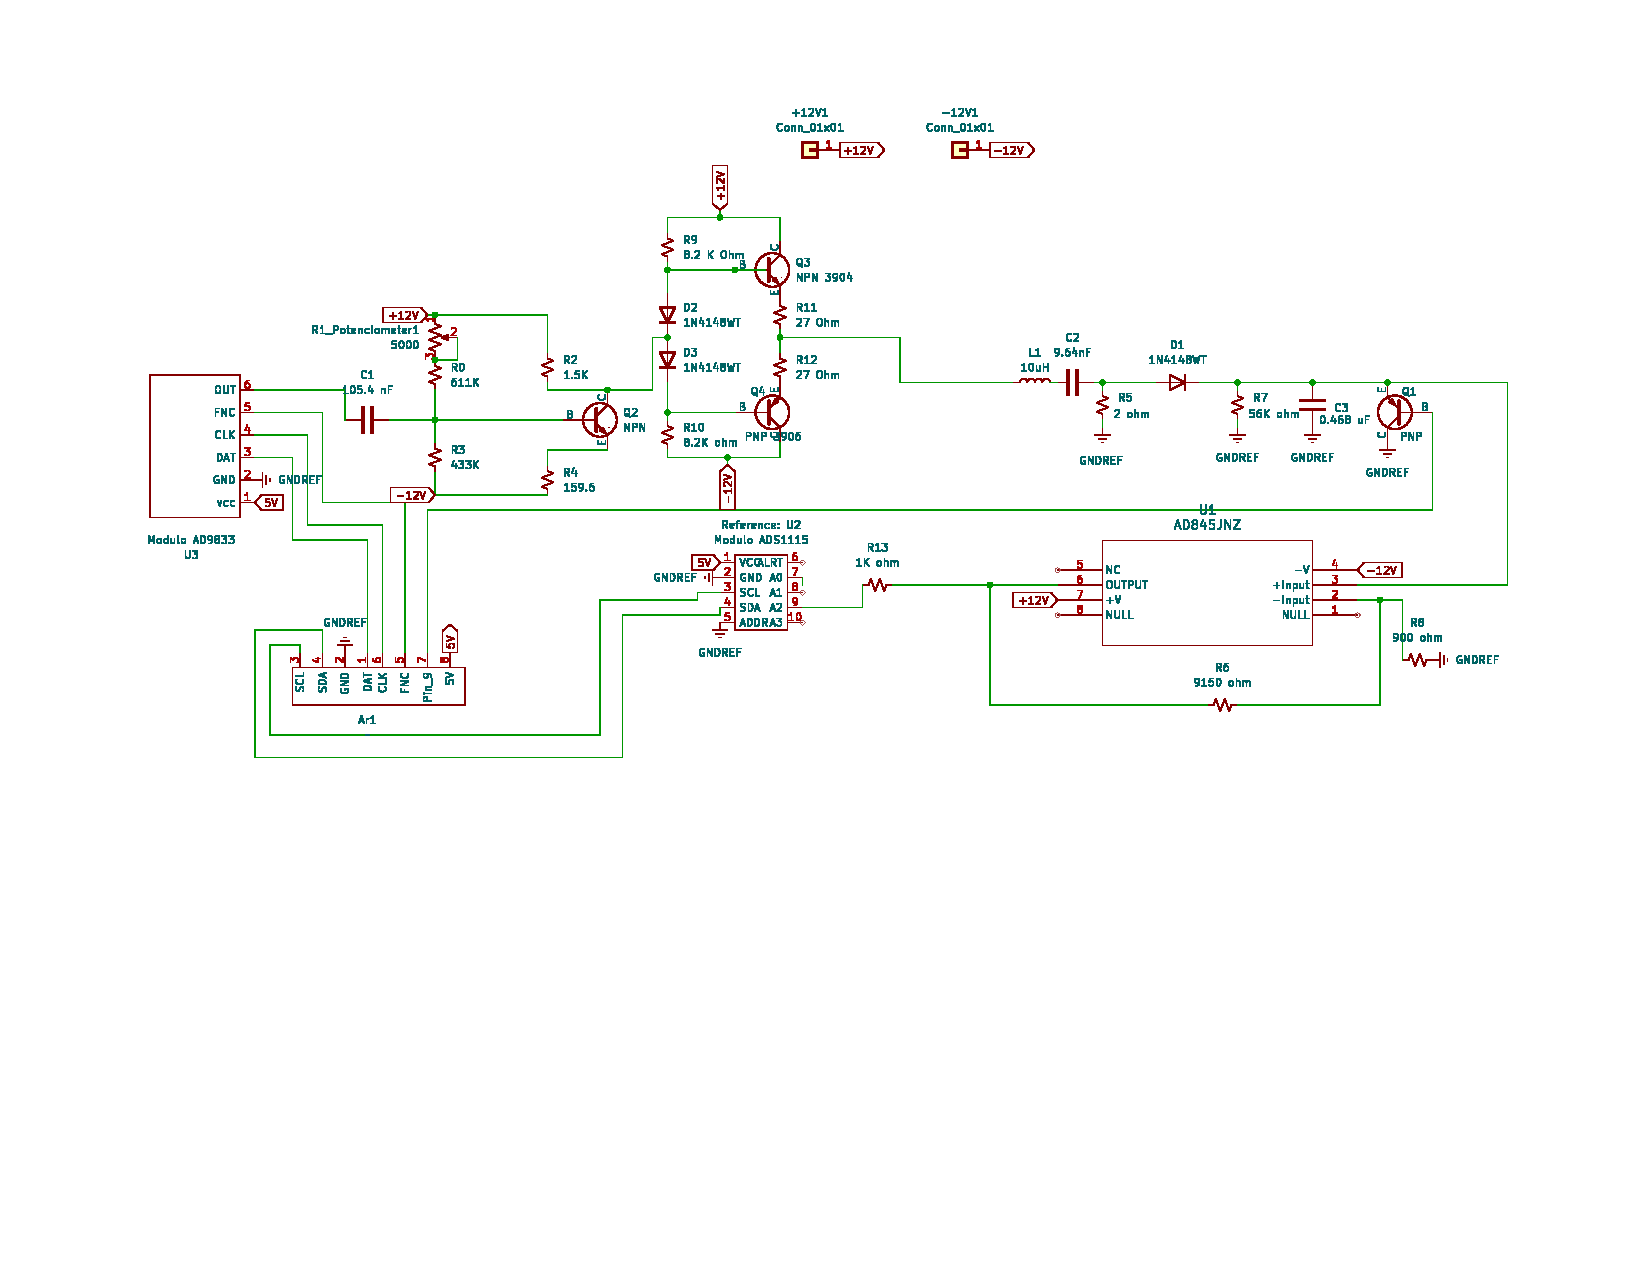
\includegraphics[width=1.0\linewidth]{esquematico-kidcad-final.pdf}
    
    \vspace{1em} % Espacio entre imagen y título
    
    % Título centrado y debajo (formato regular sin negritas según norma USB)
    \caption{Diagrama esquemático completo del prototipo conectado en serie diseñado en KiCad.}
    \label{fig:esquema_completo}
\end{sidewaysfigure}



\chapter{Matemática detrás del ajuste por ODR} % Título centrado y en negrita según norma

\label{ape:odr}

% =====================================================================
\section{ODR — Regresión Ortogonal de Distancias: ¿cómo funciona?}

El ajuste usando ODR busca los parámetros $\boldsymbol{\beta}$ y las correcciones $\delta_i$ que minimicen la suma ponderada de los cuadrados de los errores de ambas variables. Dicha función a minimizar es:

\begin{equation}
    S = \sum_{i=1}^{N} \left( \frac{\epsilon_i^2}{d_{y_i}^2} + \frac{\delta_i^2}{d_{x_i}^2} \right) \label{eq:S}
\end{equation}

de modo que si la función de ajuste es $F$, entonces se cumplen las siguientes restricciones para cada punto $i$:
\begin{equation}
    y_i - \epsilon_i = F\!\left(x_i - \delta_i\,,\, \boldsymbol{\beta}\right) \label{eq:restriccion}
\end{equation}

donde
\begin{itemize}
    \item $\epsilon_i$: corrección a cada $y_i$ medido.
    \item $\delta_i$: corrección a cada $x_i$ medido.
    \item $d_{x_i},\, d_{y_i}$: desviaciones estándar (o pesos) que representan la incertidumbre de los datos.
\end{itemize}

En nuestro caso la función $f$ es la función Lorentziana:
\begin{equation}
    F(x) = \frac{A}{(x - x_0)^2 + \gamma^2} + \text{offset} \label{eq:lorentz}
\end{equation}

de modo que los parámetros de ajuste están dados por el vector
\begin{equation}
    \boldsymbol{\beta} = \left(x_0,\, A,\, \gamma,\, \text{offset}\right) \label{eq:beta}
\end{equation}

En \texttt{scipy}, con la función \texttt{RealData(x, y, sx=sx, sy=sy)} se incluyen los valores del error de medición asociado a cada punto $x_i$ e $y_i$ como los correspondientes pesos en la ecuación de sumatoria \eqref{eq:S}:
\begin{equation}
    d_{x_i} = s_{x_i} \qquad \text{y} \qquad d_{y_i} = s_{y_i} \label{eq:pesos}
\end{equation}

de modo que un punto con un error asociado muy grande contribuye menos que uno con error menor, ya que la relación es inversa. Esto garantiza que los puntos más precisos tengan una aproximación de la curva de ajuste más cercana a ellos.

% =====================================================================
\subsection{Ajuste de \texorpdfstring{$\boldsymbol{\beta}$}{beta}}

El ODR en \texttt{scipy} usa una versión modificada del algoritmo Levenberg-Marquardt, el cual hace de forma simultánea lo siguiente:

\begin{enumerate}
    \item \textbf{Estima los errores} de cada punto $x_i$, es decir el valor $\delta_i$ que se aleja la curva ajustada al punto $x_i$.

    \item \textbf{Linealización:} Se trabaja con la expansión de Taylor de primer orden de la función $f$ al rededor de la solución $\boldsymbol{\beta}$ y $\boldsymbol{\delta}$ en evaluación.

    \item \textbf{Resolución del Sistema:} Como este algoritmo trata las correcciones $\delta_i$ como incógnitas adicionales, se plantea un sistema de ecuaciones de $4 + N$ incógnitas. Este se consigue al sustituir \eqref{eq:restriccion} en \eqref{eq:S} y aplicar la versión linealizada de la función $F$. Aquí podemos definir:
\end{enumerate}

\begin{align}
    r_i &= y_i - F(x_i, \hat{\boldsymbol{\beta}}) \tag{5.1} \label{eq:residuo}
    && \text{residuo con el punto actual}\\[6pt]
    j_i^T &= \left.\frac{\partial F}{\partial \boldsymbol{\beta}^T}\right|_{x_i,\,\hat{\boldsymbol{\beta}}} \tag{5.2} \label{eq:jacobfila}
    && \text{fila }i\text{ del jacobiano, vector }1\times p\\[6pt]
    d_i &= \left.\frac{\partial F}{\partial x}\right|_{x_i,\,\hat{\boldsymbol{\beta}}} \tag{5.3} \label{eq:sensib}
    && \text{sensibilidad local en }x\\[6pt]
    \Delta\boldsymbol{\beta} &= \boldsymbol{\beta} - \hat{\boldsymbol{\beta}} \tag{5.4} \label{eq:paso}
    && \text{paso de actualización}
\end{align}

(Los elementos \eqref{eq:jacobfila}–\eqref{eq:paso} son los parámetros de la expansión de Taylor.)

Así, la sustitución de la linealización queda:
\begin{equation}
    S \approx \sum_{i=1}^{N} \left[ \frac{\left(r_i - j_i^T \Delta\boldsymbol{\beta} + d_i\,\delta_i\right)^2}{\sigma_{y_i}^2} + \frac{\delta_i^2}{\sigma_{x_i}^2} \right] \label{eq:S_lin}
\end{equation}

Buscando eliminar a $\delta_i$ se asume que $\partial S / \partial \delta_i = 0$, lo cual permite reescribir:
\begin{equation}
    \delta_i = \frac{d_i\,\sigma_{x_i}^2}{\sigma_{y_i}^2 + d_i^2\,\sigma_{x_i}^2}\left(r_i - j_i^T \Delta\boldsymbol{\beta}\right) \label{eq:delta}
\end{equation}

Así que al sustituir \eqref{eq:delta} en \eqref{eq:S_lin} se tiene:
\begin{equation}
    S_{\text{red}}(\Delta\boldsymbol{\beta}) = \sum_{i=1}^{N} \frac{\left(r_i - j_i^T \Delta\boldsymbol{\beta}\right)^2}{\sigma_{y_i}^2 + d_i^2\,\sigma_{x_i}^2}
\end{equation}

Aquí se puede definir el \textbf{peso efectivo} de cada punto como
\begin{equation}
    w_i = \frac{1}{\sigma_{y_i}^2 + d_i^2\,\sigma_{x_i}^2}
\end{equation}

entonces
\begin{equation}
    S_{\text{red}}(\Delta\boldsymbol{\beta}) = \sum_{i=1}^{N} w_i\left(r_i - j_i^T \Delta\boldsymbol{\beta}\right)^2 \label{eq:Sred}
\end{equation}

Esto último es lo que se conoce con un problema de mínimos cuadrados ponderados en $\Delta\boldsymbol{\beta}$.

Por último se hace la minimización considerando $\partial S_{\text{red}} / \partial\Delta\boldsymbol{\beta} = 0$ pero de forma matricial, de modo que el sistema de ecuaciones que se resuelve es:
\begin{equation}
    \left(\mathbb{J}^T W \mathbb{J} + \lambda\,\mathrm{diag}\!\left(\mathbb{J}^T W \mathbb{J}\right)\right)
    \begin{pmatrix}\Delta\boldsymbol{\beta}\\ \Delta\boldsymbol{\delta}\end{pmatrix}
    = -\mathbb{J}^T W\,\mathbf{r} \label{eq:sistema}
\end{equation}

Note que el término que tiene $\lambda$ es un término de regularización agregado por Levenberg-Marquardt, el cual penaliza los pasos grandes. En \eqref{eq:sistema} tenemos:
\begin{itemize}
    \item $\mathbb{J}$: la matriz Jacobiana ($N \times p$)
    \item $W$: la matriz de pesos ($N \times N$)
    \item $\mathbf{r}$: residuos $N \times 1$
    \item $\Delta\boldsymbol{\beta}$: corrección a los parámetros ($p \times 1$)
\end{itemize}

% =====================================================================
\section{Confiabilidad del resultado del ODR}

La matriz de covarianza es la herramienta que usa \texttt{scipy} para determinar que tan confiables son los parámetros encontrados. Normalmente esta matriz contiene en su diagonal la varianza de cada parámetro; así la raíz cuadrada de estos valores son los errores estándar que arroja \texttt{scipy}. Y en el resto de los elementos de la matriz está la covarianza o correlación entre los parámetros:

\begin{equation}
    \mathrm{Cov} = \begin{pmatrix} \mathrm{Var}(\beta_1) & \mathrm{Cov}(\beta_1,\beta_2) \\ \mathrm{Cov}(\beta_2,\beta_1) & \mathrm{Var}(\beta_2) \end{pmatrix}
\end{equation}

Para el caso que estamos tratando, la matriz de covarianza está dada por:
\begin{equation}
    \mathrm{Cov}(\hat{\boldsymbol{\beta}}) = \left(\mathbb{J}^T W \mathbb{J}\right)^{-1} \label{eq:cov}
\end{equation}

A nosotros nos interesa un solo elemento de esa matriz: la varianza de $x_0$. Para poder calcularla sin hacer la inversa explícitamente podemos descomponer la matriz por bloques:
\begin{equation}
    \mathbb{J}^T W \mathbb{J} = \begin{pmatrix} \left[\mathbb{J}^T W \mathbb{J}\right]_{x_0 x_0} & \mathbf{c}^T \\ \mathbf{c} & \mathbb{B} \end{pmatrix} \label{eq:bloques}
\end{equation}

donde $\left[\mathbb{J}^T W \mathbb{J}\right]_{x_0 x_0}$ es justamente el elemento correspondiente al parámetro $x_0$ que nos interesa, $\mathbf{c}$ es el vector de acoplamiento de $x_0$ con los otros 3 parámetros, y $\mathbb{B}$ la submatriz $3\times 3$ que contiene el resto de elementos.

\subsection*{Complemento de Schur}

Sea $M$ una matriz cuadrada con dimensiones $(n+m)\times(n+m)$ partida en bloques más pequeñas:
\begin{equation}
    M_{(n+m)\times(n+m)} = \begin{pmatrix} A_{n\times n} & B_{n\times m} \\ C_{m\times n} & D_{m\times m} \end{pmatrix}
\end{equation}

Con $D$ invertible, se define el complemento de Schur del bloque $D$ de la matriz $M$ como $A - BD^{-1}C = S$. Se tiene que:
\begin{equation}
    \left[M^{-1}\right]_{11} = S^{-1}
\end{equation}

Entonces esta propiedad la podemos usar para obtener el elemento que necesitamos:
\begin{equation}
    \mathrm{Var}(x_0) = \left[\left(\mathbb{J}^T W \mathbb{J}\right)^{-1}\right]_{x_0 x_0} = \frac{1}{\left[\mathbb{J}^T W \mathbb{J}\right]_{x_0 x_0} - \mathbf{c}^T \mathbb{B}^{-1} \mathbf{c}} \label{eq:var_schur}
\end{equation}

% =====================================================================
\subsection{Elementos del Jacobiano}

Ahora escribimos todos los elementos del jacobiano. Para la diagonal de $\mathbb{J}$ hacemos las derivadas parciales de \eqref{eq:lorentz}, con el fin de simplificar introducimos la siguiente notación:
\begin{equation}
    u_i = x_i - x_0 \qquad D_i = u_i^2 + \gamma^2
\end{equation}

así derivamos parcialmente:
\begin{align}
    \mathbb{J}_{i,x_0} &= \frac{2A\,u_i}{D_i^2} &
    \mathbb{J}_{i,A} &= \frac{1}{D_i} &
    \mathbb{J}_{i,\gamma} &= \frac{-2A\,\gamma}{D_i^2} &
    \mathbb{J}_{i,\text{off}} &= 1
\end{align}

Como $\mathbb{J}^T W \mathbb{J}$ es $4\times4$ simétrica, entonces tiene 10 elementos independientes. Para cada elemento se cumple:
\begin{equation}
    \left[\mathbb{J}^T W \mathbb{J}\right]_{ab} = \sum_{i=1}^{N} w_i\,\mathbb{J}_{i,a}\,\mathbb{J}_{i,b}
\end{equation}

entonces en la diagonal:
\begin{align}
    \left[\mathbb{J}^T W \mathbb{J}\right]_{x_0 x_0} &= \sum_{i=1}^{N} \frac{4A^2 u_i^2}{D_i^4}\,w_i &
    \left[\mathbb{J}^T W \mathbb{J}\right]_{AA} &= \sum_{i=1}^{N} \frac{w_i}{D_i^2} \nonumber\\[4pt]
    \left[\mathbb{J}^T W \mathbb{J}\right]_{\gamma\gamma} &= \sum_{i=1}^{N} \frac{-4A^2\gamma^2}{D_i^4}\,w_i &
    \left[\mathbb{J}^T W \mathbb{J}\right]_{\text{off\,off}} &= \sum_{i=1}^{N} w_i \label{eq:diagonal}
\end{align}

y el resto de elementos

\begin{align}
    \left[\mathbb{J}^T W \mathbb{J}\right]_{A x_0} &= \sum_{i=1}^{N} \frac{2A\,u_i\,w_i}{D_i^3} &
    \left[\mathbb{J}^T W \mathbb{J}\right]_{A\gamma} &= \sum_{i=1}^{N} \frac{-2A\,\gamma\,w_i}{D_i^3} \nonumber\\[4pt]
    \left[\mathbb{J}^T W \mathbb{J}\right]_{A\,\text{off}} &= \sum_{i=1}^{N} \frac{w_i}{D_i} &
    \left[\mathbb{J}^T W \mathbb{J}\right]_{x_0\gamma} &= \sum_{i=1}^{N} \frac{-4A^2\gamma u_i\,w_i}{D_i^4} \nonumber\\[4pt]
    \left[\mathbb{J}^T W \mathbb{J}\right]_{x_0\,\text{off}} &= \sum_{i=1}^{N} \frac{2A\,u_i\,w_i}{D_i^2} &
    \left[\mathbb{J}^T W \mathbb{J}\right]_{\gamma\,\text{off}} &= \sum_{i=1}^{N} \frac{-2A\,\gamma\,w_i}{D_i^2} \label{eq:fuera_diag}
\end{align}

% =====================================================================
\subsubsection{Consideraciones}

Digamos que los errores son homogéneos: $\sigma_{x_i} = \sigma_x$, $\sigma_{y_i} = \sigma_y$. Esto implica en el experimento que todos los puntos se midieron con igual precisión, lo cual es de esperar normalmente si se usa el mismo instrumento para todas las medidas. Asumimos también una distribución uniforme de los $N$ puntos entre $x_0 - l$ y $x_0 + l$. Por último, en el límite continuo las sumas se convierten en integrales:
\begin{equation}
    \sum_{i=1}^{N} w_i\,\mathbb{J}_{i,a}\,\mathbb{J}_{i,b} \approx \frac{N}{2l} \int_{-l}^{l} w(u)\,\mathbb{J}_{a}(u)\,\mathbb{J}_{b}(u)\,du \label{eq:integral}
\end{equation} 

Para los pesos recordamos que $w_i = \dfrac{1}{\sigma_{y_i}^2 + d_i^2\,\sigma_{x_i}^2}$; si consideramos (5.4):
\begin{equation}
    d_i = \left.\frac{\partial f}{\partial x}\right|_{x_i} = \frac{-2A\,u_i}{D_i^2} = \frac{4A^2 u^2}{(u^2+\gamma^2)^4}
\end{equation}

entonces si $|u| \gg \gamma$ se tiene que $d_i \to 0$ $\therefore$ $w_i \approx \dfrac{1}{\sigma_y^2}$, y si $u \approx 0$ también $d_i \to 0$ y $w \to 1/\sigma_y^2$, así que asumimos la sustitución de $w_i \approx 1/\sigma_y^2$ como una aproximación.

Para resolver las integrales se hace el cambio $u = \gamma\tan\theta$, lo cual permite resolver las integrales de forma directa:
\begin{equation}
    I_n = \int_{-\infty}^{\infty} \frac{du}{(u^2+\gamma^2)^n} = \frac{\pi}{\gamma^{2n-1}} \frac{(2n-3)!!}{(2n-2)!!}
\end{equation}

Las 4 primeras soluciones son:
\begin{equation}
    I_1 = \frac{\pi}{\gamma} \qquad I_2 = \frac{\pi}{2\gamma^3} \qquad I_3 = \frac{3\pi}{8\gamma^5} \qquad I_4 = \frac{5\pi}{16\gamma^7}
\end{equation}

La otra integral que aparece tiene $u$ en el numerador; sin embargo al ser simétrica la Lorentziana en $u$, las potencias impares se anulan:
\begin{equation}
    \int_{-\infty}^{\infty} \frac{u^{2k+1}}{(u^2+\gamma^2)^n}\,du = 0
\end{equation}

% =====================================================================
\subsection{Matriz final de \texorpdfstring{$\mathbb{J}^T W \mathbb{J}$}{J^T W J}}

Usando las consideraciones anteriores, integrando las ecuaciones \eqref{eq:diagonal}:

\begin{align}
    \left[\mathbb{J}^T W \mathbb{J}\right]_{x_0 x_0} &\approx \frac{N A^2 \pi}{8l\sigma_y^2\gamma^5} \\[4pt]
    \left[\mathbb{J}^T W \mathbb{J}\right]_{AA} &\approx \frac{N\pi}{2l\sigma_y^2\gamma} \\[4pt]
    \left[\mathbb{J}^T W \mathbb{J}\right]_{\gamma\gamma} &\approx -\frac{5}{8}\frac{A^2 N\pi}{\sigma_y^2 l\gamma^5} \\[4pt]
    \left[\mathbb{J}^T W \mathbb{J}\right]_{\text{off\,off}} &= \frac{N}{\sigma_y^2}
\end{align}

y en las ecuaciones \eqref{eq:fuera_diag}:

\begin{align}
    \left[\mathbb{J}^T W \mathbb{J}\right]_{A x_0} &\approx 0 \\
    \left[\mathbb{J}^T W \mathbb{J}\right]_{A\,\text{off}} &\approx \frac{N}{\sigma_y^2 2l}\cdot\frac{\pi}{\gamma} \\
    \left[\mathbb{J}^T W \mathbb{J}\right]_{x_0\,\text{off}} &\approx 0 \\
    \left[\mathbb{J}^T W \mathbb{J}\right]_{A\gamma} &\approx -\frac{3}{4}\frac{AN\pi}{\sigma_y^2 l\gamma^4} \\
    \left[\mathbb{J}^T W \mathbb{J}\right]_{x_0\gamma} &\approx 0 \\
    \left[\mathbb{J}^T W \mathbb{J}\right]_{\gamma\,\text{off}} &\approx -\frac{AN\pi}{2\sigma_y^2 l\gamma^2}
\end{align}

Entonces la matriz $\mathbb{J}^T W \mathbb{J}$ es:

\begin{equation}
    \mathbb{J}^T W \mathbb{J} \approx \frac{N}{\sigma_y^2}
    \begin{pmatrix}
        \dfrac{A^2\pi}{8l\gamma^5} & 0 & 0 & 0 \\[10pt]
        0 & \dfrac{\pi}{2l\gamma} & \dfrac{-3A\pi}{4l\gamma^4} & \dfrac{\pi}{4l\gamma} \\[10pt]
        0 & \dfrac{-3A\pi}{4l\gamma^4} & \dfrac{-5A^2\pi}{8l\gamma^5} & \dfrac{-A\pi}{2l\gamma^2} \\[10pt]
        0 & \dfrac{\pi}{4l\gamma} & \dfrac{-A\pi}{2l\gamma^2} & 1
    \end{pmatrix}
    \label{eq:matrizfinal}
\end{equation}

% =====================================================================
\subsection{Aplicando el complemento de Schur}

Vemos que debido a la simetría de la Lorentziana, el vector $\mathbf{c}$ solo tiene ceros; por lo tanto el complemento de Schur \eqref{eq:var_schur} queda así:

\begin{equation}
    \mathrm{Var}(x_0) = \left[\left(\mathbb{J}^T W \mathbb{J}\right)^{-1}\right]_{x_0 x_0}
    = \frac{1}{\left[\mathbb{J}^T W \mathbb{J}\right]_{x_0 x_0} - \mathbf{c}^T \mathbb{B}^{-1} \mathbf{c}}
    = \frac{1}{\left[\mathbb{J}^T W \mathbb{J}\right]_{x_0 x_0}}
\end{equation}

\begin{equation}
    \boxed{\mathrm{Var}(x_0) = \frac{1}{\dfrac{N}{\sigma_y^2}\cdot\dfrac{A^2\pi}{8l\gamma^5}} = \frac{8l\gamma^5\sigma_y^2}{NA^2\pi}} \label{eq:var_final}
\end{equation}

Para que este resultado sea cierto es necesario que:
\begin{itemize}
    \item Todos los errores originales de las medidas sean iguales.
    \item Los $N$ puntos estén distribuidos de forma simétrica a cada lado del máximo de la curva.
    \item Así mismo los puntos se distribuyen desde $x_0 - l$ hasta $x_0 + l$, donde $l$ es lo suficientemente grande para abarcar parte de la curva que se hace cero (esto para que la aproximación $w_i \approx 1/\sigma_y^2$ tenga sentido, al igual que la integración en el infinito).
    \item La curva sí tenga una forma simétrica, es decir que los datos se ajusten bien a la curva de Lorentz.
\end{itemize}




\end{document}
